%%Copyright 2021. Any replication of this document is permissible. The primary package of this document is from cjquines%%

%%PRIMARY PREAMBLE%%
\documentclass[11pt,paper=letter]{scrartcl}
\usepackage[boxthm, parskip]{cjquines}
\usepackage{jrdobaob}
\usepackage{enumitem}
\usepackage{incgraph,tikz}


\begin{document}

\incgraph[documentpaper,
  overlay={\node[red] at (page.center) {\Huge };}]
  [width=\paperwidth,height=\paperheight]{Covers/2.png}

\newpage

\title{2022 PMO Write-ups (Solutions)}
\author{\joshbluebf{Philippine Mathematical Olympiad Write-Ups Series}}
\date{February 19, 2022} 

\maketitle
\setlength{\unitlength}{1in}
\begin{picture}(2,0)
  \put(0.95,1.20){\hbox{
\includegraphics[width=4.5in]{JOSH ROBERT OBAOB (3).png}}}
\end{picture}

\vspace{-2.5em}

{\small The  \joshbf{24th Philippine Mathematical Olympiad Qualifying Stage} was held on February 19, 2022 virtually. It was participated by high school students from different regions around the Philippines. These elites were selected by their respective schools. The PMO Qualifying Stage examination paper is divided into two parts: \textbf{PART I} with 15 items (2 points each) and \textbf{PART II} with 10 items (5 points each). Hence, the exam has total of 80 points and has total of 25 items. Since this is my write-up, I will compile all of the problems here so that you can see the questions (and you may try some problems if you want to) first before the solutions. Because of that, the article is divided into two parts: \joshbluebf{CHAPTER I (Questions)} and \joshbluebf{CHAPTER II (Solutions)}. Should you see any typos and errors, feel free to contact me at \mailto{jrdobaob@addu.edu.ph}, or at \mailto{joscilleo@gmail.com}.}

\vspace{-2.5em}

\tableofcontents

\newpage

\section{The 24th PMO Questions}

\textbf{PART I.} Choose the best answer. Figures are not drawn to scale. Each correct answer is worth two points. \textit{(Some of the questions have a different wording than the original PMO version)}

\begin{enumerate}[label=\textbf{\arabic*}.]
    \item Let $XZ$ be a diameter of circle $\omega$. Let $Y$ be a point of $XZ=7$ and $YZ=1.$ Let $W$ be a point on the circle such that $WY$ is perpendicular to $XZ$. Find $WY^2$.
    
    \fourch{7}{8}{10}{25}
    
    \item How many five-digit numbers containing of the digits $1,2,3,4,5$ and these digits should be distinct that are multiples of 24?
    
    \fourch{8}{10}{12}{20}
    
    \item A lattice is a point $(x,y)$ where $x$ and $y$ are both integers. Find the number of lattice points that lie on the closed line segment whose endpoints are $(2002, 2022)$ and $(2022, 2202).$
    
    \fourch{20}{21}{22}{23}
    
    \item Find the value of $1 + 2\omega + 3\omega^2 + 4\omega^3 + 5\omega^4$ such that $\omega \neq -1$ is a complex root of $x^3 +1 = 0$.
    
    \fourch{3}{$-4$}{5}{$-6$}
    
    \item How many ending zeroes does the decimal expansion of $2022!$ have?
    
    \fourch{404}{484}{500}{503}


   \item Two tigers, Alice and Betty, run in the same direction around a circular track of circumference 400 meters. Alice runs at a speed of 10 m/s and Betty runs at a speed of 15 m/s. Betty gives Alice a 40 meter headstart before they both start running. After 15 minutes, how many items will they have passed each other?

    \fourch{9}{10}{11}{12}
    
   \item Suppose $a,b,c$ are the roots of the polynomial $x^3 +2x^2 + 2$. Let $f$ be the polynomial with the leading coefficient of 1, whose roots are $a^2, b^2, c^2$. Find $f(1).$
   
   \fourch{$-17$}{$-16$}{$-15$}{$-14$}
   
   \item Let $I$ be the center of the incircle of the triangle $ABC.$ Suppose the this incircle has radius 3, and $AI =5.$ If the area of the triangle is $2022,$ what is the length of $BC$?
   
   \fourch{670}{672}{1340}{1344}
   
   \newpage
   
   \item A square is divided into eight right triangles. Find the number of ways to shade three triangles such that none of these triangles share a common edge/side.
   
   \begin{center}
 


\tikzset{every picture/.style={line width=0.75pt}} %set default line width to 0.75pt        

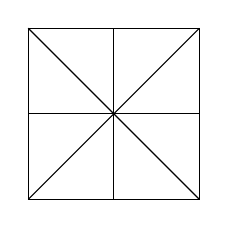
\begin{tikzpicture}[x=0.75pt,y=0.75pt,yscale=-1,xscale=1]
%uncomment if require: \path (0,300); %set diagram left start at 0, and has height of 300

%Shape: Rectangle [id:dp8556957742682403] 
\draw   (454,107) -- (536.44,107) -- (536.44,189.44) -- (454,189.44) -- cycle ;
%Straight Lines [id:da21067191751901837] 
\draw    (454,107) -- (536.44,189.44) ;
%Straight Lines [id:da5280233543074735] 
\draw    (536.44,107) -- (454,189.44) ;
%Straight Lines [id:da63365618636624] 
\draw    (536.44,189.44) -- (454,189.44) ;
%Straight Lines [id:da6745624615391608] 
\draw    (454,107) -- (536.44,107) ;
%Straight Lines [id:da9513304053736429] 
\draw    (454,148.22) -- (536.44,148.22) ;
%Straight Lines [id:da2685330817340721] 
\draw    (495.22,189.44) -- (495.22,107) ;




\end{tikzpicture}
   \end{center}
   
   \fourch{12}{16}{24}{30}
   
\item The numbers $2,b,c,d,72$ are listed in increasing order so that $2,b,c$ form an arithmetic sequence while $b,c,d$ form a geometric sequence, and $c,d,72$ form a harmonic sequence (that is, a sequence whose reciprocals of its terms form an arithmetic sequence). What is the value of $b+c.$

\fourch{7}{13}{19}{25}

\item How many positive integers $n<2022$ are there for which the sum of the odd positive divisors of $n$ is 24?

\fourch{7}{8}{14}{15}

\item Call a whole number \textit{ordinary} if the product of its digits is less than the sum of its digits. How many \textit{ordinary} numbers from the set $\{1,2,3,...,999\}$?

\fourch{151}{162}{230}{241}

\item What is the area of the shaded region of the square below?

\begin{center}



\tikzset{every picture/.style={line width=0.75pt}} %set default line width to 0.75pt        

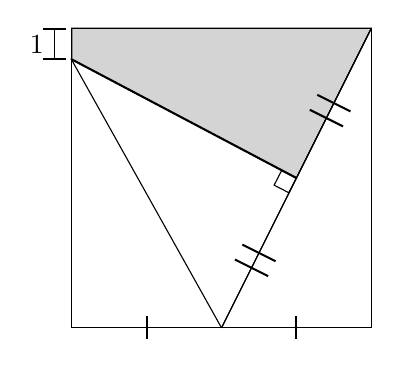
\begin{tikzpicture}[x=0.75pt,y=0.75pt,yscale=-1,xscale=1]
%uncomment if require: \path (0,572); %set diagram left start at 0, and has height of 572

%Shape: Polygon [id:ds5650543958578815] 
\draw  [color={rgb, 255:red, 0; green, 0; blue, 0 }  ,draw opacity=1 ][fill={rgb, 255:red, 212; green, 212; blue, 212 }  ,fill opacity=1 ] (243.02,245.18) -- (387.34,245.18) -- (351.26,317.34) -- (242.8,260.07) -- (243.07,259.26) -- cycle ;
%Shape: Rectangle [id:dp6795345054552426] 
\draw   (243.02,245.18) -- (387.34,245.18) -- (387.34,389.5) -- (243.02,389.5) -- cycle ;
%Straight Lines [id:da192908054306685] 
\draw    (387.34,389.5) -- (243.02,389.5) ;
%Straight Lines [id:da8685436559885313] 
\draw    (387.34,245.18) -- (315.18,389.5) ;
%Straight Lines [id:da42661267614407583] 
\draw [line width=0.75]    (351.26,317.34) -- (242.8,260.07) ;
%Shape: Rectangle [id:dp13649351225462447] 
\draw   (344.17,313.7) -- (351.26,317.34) -- (347.62,324.43) -- (340.53,320.79) -- cycle ;
%Straight Lines [id:da3751189931075172] 
\draw    (351.26,317.34) -- (315.18,389.5) ;
\draw [shift={(333.22,353.42)}, rotate = 296.57] [color={rgb, 255:red, 0; green, 0; blue, 0 }  ][line width=0.75]    (0,8.94) -- (0,-8.94)(-8.04,8.94) -- (-8.04,-8.94)   ;
%Straight Lines [id:da23660260364554286] 
\draw    (387.34,245.18) -- (351.26,317.34) ;
\draw [shift={(369.3,281.26)}, rotate = 296.57] [color={rgb, 255:red, 0; green, 0; blue, 0 }  ][line width=0.75]    (0,8.94) -- (0,-8.94)(-8.04,8.94) -- (-8.04,-8.94)   ;
%Straight Lines [id:da7038593183497226] 
\draw    (242.8,260.07) -- (315.18,389.5) ;

%Straight Lines [id:da5829046438230716] 
\draw    (234.88,245.61) -- (234.88,259.83) ;
\draw [shift={(234.88,259.83)}, rotate = 270] [color={rgb, 255:red, 0; green, 0; blue, 0 }  ][line width=0.75]    (0,5.59) -- (0,-5.59)   ;
\draw [shift={(234.88,245.61)}, rotate = 270] [color={rgb, 255:red, 0; green, 0; blue, 0 }  ][line width=0.75]    (0,5.59) -- (0,-5.59)   ;

%Straight Lines [id:da6956801139387325] 
\draw    (243.02,389.5) -- (315.18,389.5) ;
\draw [shift={(279.1,389.5)}, rotate = 180] [color={rgb, 255:red, 0; green, 0; blue, 0 }  ][line width=0.75]    (0,5.59) -- (0,-5.59)   ;
%Straight Lines [id:da00508777911562408] 
\draw    (315.18,389.5) -- (387.34,389.5) ;
\draw [shift={(351.26,389.5)}, rotate = 180] [color={rgb, 255:red, 0; green, 0; blue, 0 }  ][line width=0.75]    (0,5.59) -- (0,-5.59)   ;

% Text Node
\draw (230.73,252.99) node [anchor=east] [inner sep=0.75pt]    {$1$};


\end{tikzpicture}
\end{center}

\fourch{7}{11}{15}{19}

\item Bryce plays a game in which he flips a fair coin repeatedly. In each flip, he obtains two tokens if the coin lands on heads, and loses one coin if it's tails. From the beginning, he has nine tokens. If after nine flips, he still retains the number of tokens he had from the beginning. Find the probability of Bryce having nine tokens at the end. 

\fourch{1/7}{1/6}{5/28}{17/84}


\newpage

\item How many ways are there to arrange the first ten positive integers such that the multiples of 2 appear in increasing order, and the multiples of 3 appear in decreasing order?

\fourch{720}{2160}{5040}{6480}

\end{enumerate}

\textbf{PART II.} All answers are positive integers. Do not use commas if there are more than 3 digits, e,g., type 1234 instead of 1,234. A fraction $a/b$ is in lowest terms if $a$ and $b$ are positive integers whose greatest common factor is 1. Each correct answer is worth five points. 

   \begin{enumerate}[resume, label=\arabic*.,font=\bfseries]
    
    \item What is the largest multiple of 7 less than 10,000 which can be expressed as the sum of squares of three consecutive numbers?
    
    \item Suppose that the polynomial $P(x) = x^3 + 4x^2 + bx +c$ has a single root $r$ and a double root $s$ for some distinct real numbers $r$ and $s$. Given that $P(-2s) = 324$, what is the sum of all possible values of $|c|$?
    
    \item Let $m$ and $n$ be relatively prime positive integers. If $m^3n^5$ has 209 positive divisors, then how many positive divisors does $m^5n^3$ have?
    
    \item Let $x$ be a positive real number. What is the maximum value of $\dfrac{2022x^2 \log(x+2022)}{\left(\log(x+2022)\right)^3 + 2x^3}$?
    
    \item Let $a,b,c$ be real numbers such that $$3ab + 2 = 6b, \quad 3bc + 2 = 5c, \quad 3ca + 2 =4a.$$
    
   Suppose the only possible values for the product $abc$ are $r/s$ and $t/u$, where $r/s$ and $t/u$ are both fractions in lowest terms. Find $r+s+t+u.$
    
    \item You roll a fair 12-sided die repeatedly. The probability that all primes show up at least once before seeing any of the other numbers can be expressed as a fraction $p/q$ in lowest terms. What is $p+q$?
    
    \item Let $PMO$ be a triangle with $PM =2$ and $\angle PMO = 120^{\circ}$. Let $B$ be a point on $PO$ such that $PM$ is perpendicular to $MB$ and suppose that $PM=BO$. The product of the lengths of the sides of the triangle can be expressed in the form $a + b\sqrt[3]{c}$, where $a,b,c$ are positive integers and $c$ is minimized. Find $a+b+c$.
    
    \item Let $ABC$ be a triangle such that the altitude from $A$, the median from $B$, and the internal angle bisector from $C$ meet at a single point. If $BC = 10$ and $CA = 15,$ find $AB^2.$
    
    \item Find the sum of all positive integers $n, 1 \leq n \leq 5000,$ which $$n^2 +2475n +2454 + (-1)^n$$is divisible by 2477. (Note that 2477 is a prime number.)
    
    \newpage
    
    \item For a real number $x$, let $\lfloor x \rfloor$ denote the greatest integer not exceeding $x$. Consider the function $$f(x,y) = \sqrt{M(M+1)}\left(|x-m|+|y-m|\right),$$ where $M = \text{max} (\lfloor x \rfloor, \lfloor y \rfloor)$ and $m = \text{min} (\lfloor x \rfloor, \lfloor y \rfloor)$. The set of all real numbers $(x,y)$ such that $2 \leq x, y \leq 2022$ and $f(x,y) \leq 2$ can be expressed as a finite union of disjoint regions in the plane. The sum of the areas of these regions can be expressed as a fraction $a/b$ in lowest terms. What is the value of $a+b?$
    
    
\end{enumerate}

\newpage

\section{Solutions}

\subsection{PART I}

Choose the best answer. Figures are not drawn to scale. Each correct answer is worth two points. \textit{(Some of the questions have a different wording than the original PMO version)}

\vspace{2mm}

\subsubsection{Item \# 1}

\begin{probboxed}
 Let $XZ$ be a diameter of circle $\omega$. Let $Y$ be a point of $XZ=7$ and $YZ=1.$ Let $W$ be a point on the circle such that $WY$ is perpendicular to $XZ$. Find $WY^2$.
    
    \fourch{7}{8}{10}{25}
\end{probboxed}

\ans{(a) 7}

\sol

\begin{center}



\tikzset{every picture/.style={line width=0.75pt}} %set default line width to 0.75pt        

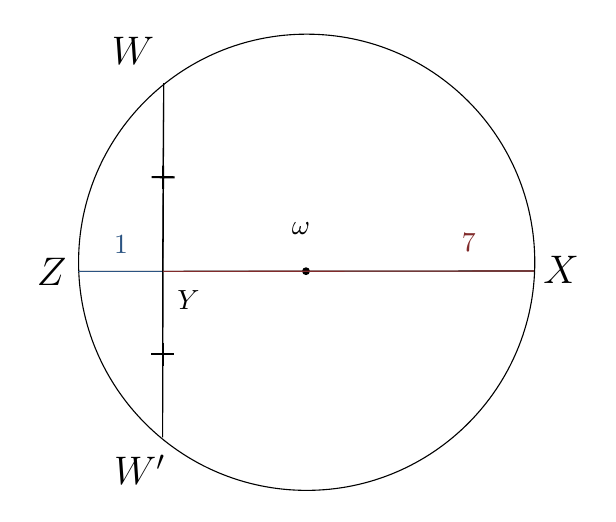
\begin{tikzpicture}[x=0.75pt,y=0.75pt,yscale=-1,xscale=1]
%uncomment if require: \path (0,326); %set diagram left start at 0, and has height of 326

%Shape: Circle [id:dp6149784346054472] 
\draw   (90,166.1) .. controls (90,105.4) and (139.2,56.2) .. (199.9,56.2) .. controls (260.6,56.2) and (309.8,105.4) .. (309.8,166.1) .. controls (309.8,226.8) and (260.6,276) .. (199.9,276) .. controls (139.2,276) and (90,226.8) .. (90,166.1) -- cycle ;
%Straight Lines [id:da46650192687471814] 
\draw    (89.75,170.5) -- (309.4,170.3) ;
\draw [shift={(199.58,170.4)}, rotate = 359.95] [color={rgb, 255:red, 0; green, 0; blue, 0 }  ][fill={rgb, 255:red, 0; green, 0; blue, 0 }  ][line width=0.75]      (0, 0) circle [x radius= 1.34, y radius= 1.34]   ;
%Straight Lines [id:da5421465876681388] 
\draw    (131,79.75) -- (130.5,250.5) ;
%Straight Lines [id:da0928503014676243] 
\draw [color={rgb, 255:red, 43; green, 83; blue, 129 }  ,draw opacity=1 ]   (89.75,170.5) -- (130.5,170.5) ;
%Straight Lines [id:da8445717459344939] 
\draw [color={rgb, 255:red, 129; green, 43; blue, 43 }  ,draw opacity=1 ]   (130.5,170.5) -- (309.4,170.3) ;
%Straight Lines [id:da9545249019950093] 
\draw    (131,79.75) -- (130.5,170.5) ;
\draw [shift={(130.75,125.13)}, rotate = 90.32] [color={rgb, 255:red, 0; green, 0; blue, 0 }  ][line width=0.75]    (-5.59,0) -- (5.59,0)(0,5.59) -- (0,-5.59)   ;
%Straight Lines [id:da03989812376987789] 
\draw    (130.5,170.5) -- (130.5,250.5) ;
\draw [shift={(130.5,210.5)}, rotate = 90] [color={rgb, 255:red, 0; green, 0; blue, 0 }  ][line width=0.75]    (-5.59,0) -- (5.59,0)(0,5.59) -- (0,-5.59)   ;

% Text Node
\draw (191.5,145.5) node [anchor=north west][inner sep=0.75pt]    {$\omega $};
% Text Node
\draw (77.05,170.63) node  [font=\Large]  {$Z$};
% Text Node
\draw (322.47,169.63) node  [font=\Large]  {$X$};
% Text Node
\draw (142.91,184.2) node    {$Y$};
% Text Node
\draw (116.24,64.08) node  [font=\Large]  {$W$};
% Text Node
\draw (119.53,266.13) node  [font=\Large]  {$W'$};
% Text Node
\draw (110.48,157.7) node    {$\textcolor[rgb]{0.17,0.33,0.51}{1}$};
% Text Node
\draw (277.98,156.7) node  [color={rgb, 255:red, 129; green, 43; blue, 43 }  ,opacity=1 ]  {$7$};


\end{tikzpicture}
\end{center}

Note that diameter $XZ$ is a chord itself and so does $W'$. We let $W'Y$ be the extension of $WY$ such that $W'$ is a point on $\omega$. By intersecting chords theorem, $WY \cdot YW' = WY^2 = XY \cdot XZ = 7 \cdot 1 = 7.$ Hence, our final answer is $7.$

\subsubsection{Item \# 2}

\begin{probboxed}
 How many five-digit numbers containing of the digits $1,2,3,4,5$ and these digits should be distinct that are multiples of 24?
    
    \fourch{8}{10}{12}{20}
\end{probboxed}

\ans{(b) 10}

\sol 

For the first solution, we are going to do some listing of numbers. Note that $24 = 8 \times 3$. So, the number must be divisible by $8$ and $3.$ Since the former is its property, this means that the last two digits must be divisible by $4.$ Without the loss of generality, we will let such number be $\overline{abcd}.$ such that $a,b,c,d \in \{1,2,3,4,5\}$. 


We will do case work here as well. Before notice that the possible values of $\overline{cd}$ that are divisible by 4 are $12, 24, 32$ and 52. Now, we have these values, we get that if the number has the last two digits of $\overline{12}$ has \fbox{4} numbers satisfying the condition, and (2) if the number has the last two digits of $\overline{24}.$, only \fbox{2}. numbers out of 3! are divisible by 24. (3) If $\overline{32}$, there are no multiples of 24 satisfying this case. Finally, for $\overline{52}$, we have \fbox{4} multiples of 24, satisfying the condition. Hence we have $4+2+4 = \fbox{10}$ numbers.

\subsubsection{Item \# 3}

\begin{probboxed}
A lattice is a point $(x,y)$ where $x$ and $y$ are both integers. Find the number of lattice points that lie on the closed line segment whose endpoints are $(2002, 2022)$ and $(2022, 2202).$
    
    \fourch{20}{21}{22}{23}
\end{probboxed}

\ans{(b) 21}

\sol

The approach is easy because you only need to find the equation of the line. To find it, we will use the point-slope form such that $$y-y_1 = m(x-x_1)$$ where $(x_1, y_1) $ is a point in the line and $m = \dfrac{y_2 - y_1}{x_2 - x_1}$ where $(x_2, y_2)$ is the other point on the line. Finding the equation gives us the guarantee that all integers $x$ will give us output integers $y$. Hence, we have \fbox{21} lattice points.

\begin{mdframed}
\begin{rem}
Try this problem from \href{http://pmo.ph/wp-content/uploads/2018/08/PMO-20-Qualifying-Round-with-answers-only.pdf}{PMO 20 Qualifying I.12}

"A lattice point is a point whose coordinates are integers. How many lattice points are strictly inside the triangle formed by the points $(0, 0), (0, 7),$and $(8, 0)$?"
\end{rem}
\end{mdframed}
\subsubsection{Item \# 4}

\begin{probboxed}
Find the value of $1 + 2\omega + 3\omega^2 + 4\omega^3 + 5\omega^4$ such that $\omega \neq -1$ is a complex root of $x^3 +1 = 0$.
    
    \fourch{3}{$-4$}{5}{$-6$}
\end{probboxed}

\ans{(d) $-6$}

\soln1

Let $S = 1 + 2\omega + 3\omega^2 + 4\omega^3 + 5\omega^4$. Notice that this is an \joshbf{arithmetico-geometric series}. In order for most of the coefficients be 1, let us make another equation by multiplying $S$ with $w.$ $$S(w) = w + 2w^2 + 3w^3 + 4w^4 + 5w^5$$ 


Subtracting the two equations, we have $S(1-w) =   1+ w + w^2 + w^3 + w^4 - 5w^5 $. Notice this equation can be rewritten as $$S = \dfrac{1 + w + w^2 + w^3 + w^4 + w^5 - 6w^5}{1-w} \Leftrightarrow \left((w^3 + 1)(1 + w + w^2) - 6w^5\right)(w) = -6w^6 = -6$$ Hence, our final answer is \fbox{$-6$}.

\begin{mdframed}
\begin{rem}
Try this problem from Mock AIME 2 2007/5: Find all complex $z$ such that $iz = 1 + \frac{2}{z} + \frac{3}{z^2} + ...$
\end{rem}
\end{mdframed}

\soln2

Another approach will be like this:

Note that $w^3 = -1$, and we have $$1 + 2w + 3w^2 -4 - 5w \implies 3w^2 -3w -3.$$

But since $w^3 + 1 = 0$ and $w \neq 1$, and $w^2 - w + 1 =0$, then $$3w^2 -3w -3 \implies 3(w^2 - w + 1) + 3(-2) = 0 - 6 = -6. $$ Hence, we got the same answer.

\begin{mdframed}
\begin{rem}
Special thanks to the former PMO National Finalist and Cedie's Mathverse's \textbf{Charles Dwight Pelaez} for this shortcut!
\end{rem}
\end{mdframed}
\subsubsection{Item \# 5}

\begin{probboxed}
How many ending zeroes does the decimal expansion of $2022!$ have?
    
\fourch{404}{484}{500}{503}
\end{probboxed}
  
 \ans{(d) 503}
 
 \sol
 
Expanding the number 2022! is too rigid. Luckily, we have one formula that can help us to solve this problem which is the Legendre's formula:

\begin{mdframed}
\begin{theorem}[Legendre's Formula]

The formula states that

\begin{equation*}
    \sum_{i=1} ^{\infty} \bigg \lfloor \dfrac{n}{p^i} \bigg \rfloor = \bigg \lfloor \dfrac{n}{p} \bigg \rfloor + \bigg \lfloor \dfrac{n}{p^2} \bigg \rfloor + \bigg \lfloor \dfrac{n}{p^3} \bigg \rfloor + \bigg \lfloor \dfrac{n}{p^4} \bigg \rfloor + ...
\end{equation*}

where $n$ is a positive integer and $p$ is a prime in the prime factorization of $n!$

\end{theorem}
\end{mdframed}

By using the formula, we will let $(n,p) = (2022, 5)$. Invoking it, we have $404 + 80 + 16 + 3 = \fbox{503}.$ And that is our final answer.

\subsubsection{Item \# 6}

\begin{probboxed}
Two tigers, Alice and Betty, run in the same direction around a circular track of circumference 400 meters. Alice runs at a speed of 10 m/s and Betty runs at a speed of 15 m/s. Betty gives Alice a 40 meter headstart before they both start running. After 15 minutes, how many items will they have passed each other?

\fourch{9}{10}{11}{12}

\end{probboxed}

\ans{(d) 12}

\sol After they start, the first meeting will happen in $\dfrac{40m }{15m/s - 10m/s}= 8s$. After that, the time taken is fixed which is $\dfrac{400m}{15m/s - 10m/s}$ before they meet again.

\vspace{2mm}

Let $x$ be the number of times they intersect through a rate of 80 seconds. Then we have $8 + 80x \leq 900$ $$8 + 80x \leq 900 \Leftrightarrow 80x \leq872 \implies x \leq \dfrac{872}{80} = 11 + \dfrac{3}{20}  $$. Since this is a rational number, then you just take the floor function and we have 11 intersections. However, we forgot one more intersection when they start once again (this time, no headstart for Alice), so we have $11 + 1 =$ \fbox{12}


\begin{mdframed}
\begin{rem}
Thanks to \joshbf{Kurt Ecaranum} for this solution!
\end{rem}
\end{mdframed}


\subsubsection{Item \# 7}

\begin{probboxed}
Suppose $a,b,c$ are the roots of the polynomial $x^3 +2x^2 + 2$. Let $f$ be the polynomial with the leading coefficient of 1, whose roots are $a^2, b^2, c^2$. Find $f(1).$
   
   \fourch{$-17$}{$-16$}{$-15$}{$-14$}
\end{probboxed}

\ans{(c) 15}

\sol

In this solution, we are going to apply Vieta's formulas. Note that $a+b+c = -2$, $ab+bc+ca = 0$, and $abc = -2$. Since we are asked to find $f(1)$, we are going to make $f(x)$: $$f(x) = x^3 - (a^2 + b^2 + c^2)x^2 + (a^2b^2+b^2c^2+c^2a^2)x - (abc)^2$$. 

\begin{itemize}
    \item To find $\sum a^2$, note that it is equivalent to $\left(\sum a\right)^2 -2\left(\sum ab\right) = (-2)^2 - 2(0) = \fbox{4}$. 
    
    \item To find $\sum a^2b^2$, note that it is equivalent to $\left(\sum ab\right)^2 -2abc\left(\sum a\right)= 0 -2(-2)(-2) = \fbox{$-8$}$. 
    
    \item Finally, $(abc)^2 = (-2)^2 = \fbox{4}$
\end{itemize}

Hence, $f(x) = x^3 -4x^2 -8x - 4$ and $f(1) = 1 - (4+8+4) = $ \fbox{$-15$}

\begin{mdframed}
\begin{rem}
Watch PMO's tutorial videos about \href{https://www.youtube.com/watch?v=yT1-mWubPxs}{Vieta's Formula (General case)} and \href{https://www.youtube.com/watch?v=M53VPK1ZnuI&t=267s}{Vieta's Formula (Quadratic case) if you want to know more.}
\end{rem}

\end{mdframed}


\subsubsection{Item \# 8}

\begin{probboxed}
Let $I$ be the center of the incircle of the triangle $ABC.$ Suppose the this incircle has radius 3, and $AI =5.$ If the area of the triangle is $2022,$ what is the length of $BC$?
   
   \fourch{670}{672}{1340}{1344}
\end{probboxed}

\ans{(a) 670}

\sol

Refer to the figure below:

\begin{center}



\tikzset{every picture/.style={line width=0.75pt}} %set default line width to 0.75pt        

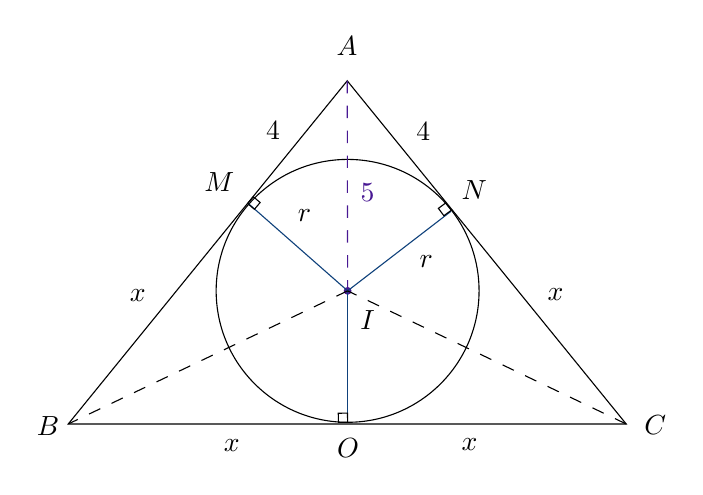
\begin{tikzpicture}[x=0.75pt,y=0.75pt,yscale=-1,xscale=1]
%uncomment if require: \path (0,379); %set diagram left start at 0, and has height of 379

%Shape: Triangle [id:dp8881483895062565] 
\draw   (488.28,35.8) -- (622.68,201.13) -- (353.88,201.13) -- cycle ;
%Shape: Circle [id:dp7026450666992561] 
\draw   (425.13,137) .. controls (425.13,102.02) and (453.49,73.67) .. (488.47,73.67) .. controls (523.44,73.67) and (551.8,102.02) .. (551.8,137) .. controls (551.8,171.98) and (523.44,200.33) .. (488.47,200.33) .. controls (453.49,200.33) and (425.13,171.98) .. (425.13,137) -- cycle ;
%Straight Lines [id:da7807899762069297] 
\draw [color={rgb, 255:red, 72; green, 24; blue, 147 }  ,draw opacity=1 ] [dash pattern={on 4.5pt off 4.5pt}]  (488.28,35.8) -- (488.47,137) ;
\draw [shift={(488.47,137)}, rotate = 89.89] [color={rgb, 255:red, 72; green, 24; blue, 147 }  ,draw opacity=1 ][fill={rgb, 255:red, 72; green, 24; blue, 147 }  ,fill opacity=1 ][line width=0.75]      (0, 0) circle [x radius= 1.34, y radius= 1.34]   ;
%Straight Lines [id:da7824427830846021] 
\draw [color={rgb, 255:red, 15; green, 65; blue, 123 }  ,draw opacity=1 ]   (538.3,98.65) -- (488.47,137) ;
%Shape: Square [id:dp040742585981685675] 
\draw   (534.86,100.81) -- (532.21,97.26) -- (535.76,94.61) -- (538.41,98.16) -- cycle ;
%Straight Lines [id:da5177289413334158] 
\draw [color={rgb, 255:red, 15; green, 65; blue, 123 }  ,draw opacity=1 ]   (440.3,94.65) -- (488.47,137) ;
%Shape: Square [id:dp38110502391852163] 
\draw   (443.08,91.67) -- (446.33,94.45) -- (443.56,97.69) -- (440.31,94.92) -- cycle ;
%Straight Lines [id:da04913887449736842] 
\draw [color={rgb, 255:red, 15; green, 65; blue, 123 }  ,draw opacity=1 ]   (488.47,137) -- (488.47,200.33) ;
%Shape: Square [id:dp771512893793528] 
\draw   (484.04,200.4) -- (483.97,195.97) -- (488.4,195.9) -- (488.47,200.33) -- cycle ;
%Straight Lines [id:da8686517924918087] 
\draw  [dash pattern={on 4.5pt off 4.5pt}]  (622.68,201.13) -- (488.47,137) ;
%Straight Lines [id:da3526056506873916] 
\draw  [dash pattern={on 4.5pt off 4.5pt}]  (488.47,137) -- (353.88,201.13) ;

% Text Node
\draw (488.19,19.2) node    {$A$};
% Text Node
\draw (636.65,201.53) node    {$C$};
% Text Node
\draw (344.16,202.07) node    {$B$};
% Text Node
\draw (498.03,151.23) node    {$I$};
% Text Node
\draw (426.69,84.68) node    {$M$};
% Text Node
\draw (549.52,88.25) node    {$N$};
% Text Node
\draw (467.73,100.87) node    {$r$};
% Text Node
\draw (526.39,122.87) node    {$r$};
% Text Node
\draw (498.06,89.87) node  [color={rgb, 255:red, 72; green, 24; blue, 147 }  ,opacity=1 ]  {$5$};
% Text Node
\draw (387.35,139.32) node    {$x$};
% Text Node
\draw (432.69,211.65) node    {$x$};
% Text Node
\draw (547.19,211.07) node    {$x$};
% Text Node
\draw (588.69,138.82) node    {$x$};
% Text Node
\draw (452.56,59.62) node    {$4$};
% Text Node
\draw (524.89,60.45) node    {$4$};
% Text Node
\draw (488.69,212.68) node    {$O$};


\end{tikzpicture}
\end{center}

Let $M, N$ and $O$ be the points of tangency of line segments $AB, AC$ and $BC.$ Let $r=3$ be the inradius of the incircle $I$. Because $AI = 5$, and $MI = IN = r$, and $\angle AMI = \angle ANI$, then by SSA, $\Delta AMI \cong \Delta AIN$, Let $x = MB \in AB$ and by theorem, $MB = BO = x$. Similarly, $NC = OC = x$. This gives us $BC = 2x$ and $\Delta ABC$ is an isosceles triangle, and $AM =AN$.

Next, recall the formula for the inradius of an incircle and that is, $$r = \dfrac{2[ABC]}{s_1 + s_2 + s_3}$$ where $[ABC]$ is the area of the $\Delta ABC$, $r$ be the radius and $s_1,s_2,s_3$ be the sides of that triangle. 

Substituting the formula gives us $\dfrac{2(2022)}{4x + 8} = 3$. Then, this gives us $x = 335 $ or $2x = BC = 670,$ and this is one of the choices.
    


Hence, our final answer is \fbox{(a) 670}.

\begin{mdframed}
\begin{rem} Try this problem from \href{https://pmo.ph/wp-content/uploads/2019/01/21st-PMO-Qualifying-Stage.pdf}{PMO 21 Qualifying II.3}

"Quadrilateral $ABCD$ has $AB = 25, BC = 60, CD = 39$, $DA = 52$, and $AC = 65$. What is the
inradius of $\Delta BCD$?"

\end{rem}
\end{mdframed}
\subsubsection{Item \# 9}

\begin{probboxed}
A square is divided into eight right triangles. Find the number of ways to shade three triangles such that none of these triangles share a common edge/side.
   
   \begin{center}
 


\tikzset{every picture/.style={line width=0.75pt}} %set default line width to 0.75pt        

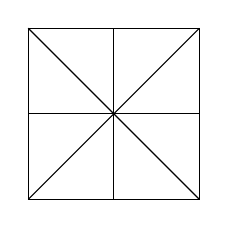
\begin{tikzpicture}[x=0.75pt,y=0.75pt,yscale=-1,xscale=1]
%uncomment if require: \path (0,300); %set diagram left start at 0, and has height of 300

%Shape: Rectangle [id:dp8556957742682403] 
\draw   (454,107) -- (536.44,107) -- (536.44,189.44) -- (454,189.44) -- cycle ;
%Straight Lines [id:da21067191751901837] 
\draw    (454,107) -- (536.44,189.44) ;
%Straight Lines [id:da5280233543074735] 
\draw    (536.44,107) -- (454,189.44) ;
%Straight Lines [id:da63365618636624] 
\draw    (536.44,189.44) -- (454,189.44) ;
%Straight Lines [id:da6745624615391608] 
\draw    (454,107) -- (536.44,107) ;
%Straight Lines [id:da9513304053736429] 
\draw    (454,148.22) -- (536.44,148.22) ;
%Straight Lines [id:da2685330817340721] 
\draw    (495.22,189.44) -- (495.22,107) ;




\end{tikzpicture}
   \end{center}
   
   \fourch{12}{16}{24}{30}
\end{probboxed}


\ans{(b) 16}

\soln1


Note that we have $\binom 83$ total ways to shade three triangles in the figure whenever they have a common edge or not. For our approach, we will do compliment counting. Counting the number of ways to shade three triangles having a common side gives us $40$ ways. Thus, we have $56-40 =$ \fbox{16} ways.

%%%  @BenedictRodil

\begin{mdframed}
\begin{rem}
Special thanks to \textbf{Benedict Rodil} for this!
\end{rem}
\end{mdframed}

\newpage

\soln2

Note that we have four smaller squares. In this case, we are going to choose 3 out of 4 so this gives us $\binom 43 = 4$. Next, we choose one of the 2 small triangles and this gives us $2^3 = 8$ and subtract 4 cases from it (the cases that make the triangles have a common side). Thus, we have $(\binom 43)(2^3 -4) = 16$.

\begin{mdframed}
\begin{rem}
Special thanks to the former PMO National Finalist and Cedie's Mathverse's \textbf{Charles Dwight Pelaez} for this shortcut!
\end{rem}

\begin{rem}
I was supposed to have my own solution here but for me, it is too abstract.
\end{rem}
\end{mdframed}



\subsubsection{Item \# 10}

\begin{probboxed}
The numbers $2,b,c,d,72$ are listed in increasing order so that $2,b,c$ form an arithmetic sequence while $b,c,d$ form a geometric sequence, and $c,d,72$ form a harmonic sequence (that is, a sequence whose reciprocals of its terms form an arithmetic sequence). What is the value of $b+c.$

\fourch{7}{13}{19}{25}
\end{probboxed}

\ans{(c) 19}

\sol From the problem, we get a system of equations: 

\begin{center}
    \begin{cases} 2b = 2 + c \\ c^2 = bd \\ \dfrac{2}{d} = \dfrac{1}{c} + \dfrac{1}{72} \end{cases}
\end{center}

From this system, the second equation can be transformed into the equation for $d$ such that $d = \dfrac{c^2}{b}$. Substitute it into the third equation, we have: $$\dfrac{2b}{c^2} = \dfrac{1}{c} + \dfrac{1}{72} \implies \dfrac{2+c}{c^2} = \dfrac{1}{c} + \dfrac{1}{72}$$. 
Solving for $c$, we have $c = 12$. Now, we can find $b$ in the first equation, and this gives us $2b = 2 + (12) = 14$. Thus, $b=7.$ Therefore $b+c = 12 + 7 = \fbox{19}.$

\begin{mdframed}

\begin{rem}
The 'surface' of the problem seems hard to be penetrated but as long as you have the basic knowledge about solving a system of equations and sequences, you can solve it in a mini-second!
\end{rem}


\begin{rem}
Try this problem from \href{http://pmo.ph/wp-content/uploads/2020/12/15th-PMO-Qualifying-Area-Stage.pdf}{PMO 15 Areas I.8}

"Let $3x, 4y, 5z$ form a geometric sequence while $\dfrac{1}{x},\dfrac{1}{y}, \dfrac{1}{z} $ form an arithmetic
sequence. Find the value of $\dfrac{x}{z} + \dfrac{z}{x}.$
\end{rem}
\end{mdframed}

\subsubsection{Item \# 11}

\begin{probboxed}
\item How many positive integers $n<2022$ are there for which the sum of the odd positive divisors of $n$ is 24?

\fourch{7}{8}{14}{15}
\end{probboxed}

\ans{(d) 15}

\sol

Note that the smallest possible positive integer that satisfies the condition is 15. Notice that $2^n \times 15$ has also the same sum of odd positive integers of 15. So, for this one, we are going to find the number of these multiples less than 2022, and computing such, we have $$2^k \leq \dfrac{674}{5} \implies k \leq 7$$. So we have 7 + 1 = 8 positive integers that satisfy the condition

Next, we have 23 and same logic applies to it which $23 \times 2^k$ must be less than 2022. So, we have $$2^k \leq \dfrac{2022}{23} \implies k \leq 6$$. So we have 6 + 1 = 7 positive integers satisfying the condition.

Therefore, we have \fbox{$15$} positive integers.

\begin{mdframed}
\begin{rem}
The solution is from Dumplet's video: \url{https://www.youtube.com/watch?v=bTX4fus5LxM}.
\end{rem}

\begin{rem}
Try this one from \href{http://pmo.ph/wp-content/uploads/2018/08/PMO-20-Qualifying-Round-with-answers-only.pdf}{PMO 20 Qualifying II.5}

"Let N be the smallest three-digit positive number with exactly 8 positive even divisors. What is the sum of the digits of N?"
\end{rem}
\end{mdframed}
\subsubsection{Item \# 12}

\begin{probboxed}
Call a whole number \textit{ordinary} if the product of its digits is less than the sum of its digits. How many \textit{ordinary} numbers from the set $\{1,2,3,...,999\}$?

\fourch{151}{162}{230}{241}
\end{probboxed}

\ans{(d) 241}

\soln1

Let us dome some casework:

\begin{itemize}
    \item For \textbf{Case 1}, that is, the number of one-digit numbers that are \textit{ordinary.}
    
     \item For \textbf{Case 2}, that is, the number of two-digit numbers that are \textit{ordinary.}
     
     \item For \textbf{Case 3}, that is, the number of three-digit numbers that are \textit{ordinary.}
\end{itemize}

For \textbf{Case 1,} we have no \textit{ordinary} numbers. For \textbf{Case 2}, numbers from $10 - 19$, numbers $20-21, 30-31, 40 - 41,..., 90-91$ satisfy the condition. Hence, we have $10 + 2(8) = \fbox{26}$ \textit{ordinary} numbers. 

For \textbf{Case 3}, let us divide the cases into subcases for 100-199, 200-299 up to 900-999. 

\begin{itemize}
    \item For $100-199$, we have numbers $100-110$, $111 - 119$, $120-122$, $130-131$, $140-141$,...,$190-191$ satisfying the condition. Hence, we have $11 + 9 + 3 + 2(7) = \fbox{37}$ \textit{ordinary} numbers.
    
    \item For $200-299$, we have numbers $200-210$, $211 - 219$, $220, 221$, $230,231$,...,$290,291$ satisfying the condition. Hence, we have $11 + 9 + 1 + 2(8) = 20 + 16 = \fbox{37}$ \textit{ordinary} numbers.
    
    \item For $300-399$, we have numbers $300-310, 311, 320, 321, 330, 340, 350, 360,...,390$ satisfying the condition. Hence, we have $11+3+7=\fbox{21}$ \textit{ordinary} numbers
    
    \item For $400-499$, we have numbers $400-410, 411, 420, 430, 440, 450, 460,...,490$ satisfying the condition. Hence, we have $12+8=\fbox{20}$ \textit{ordinary} numbers
    
    \item For $500-599$, we have numbers $500-510, 511, 520, 530, 540, 550, 560,...,590$ satisfying the condition. Hence, we have $12+8=\fbox{20}$ \textit{ordinary} numbers
    
     \item For $600-699$, we have numbers $600-610, 611, 620, 630, 540, 550, 560,...,590$ satisfying the condition. Hence, we have $12+8=\fbox{20}$ \textit{ordinary} numbers
    
    Notice that subcases $500-599,600-699,...,900-999$ make up the $20(6) =120$ \textit{ordinary} numbers. 
    
    $\therefore$ Adding all of the cases, we have $26 + 2(37) + 21 + 120 = \fbox{241}$ numbers
\end{itemize}

\soln2

If you have a head like me, you would do complimentary counting. Just put in your mind that you have $999$ numbers and you should eliminate the following numbers:

\begin{itemize}
    \item Numbers that both the sum and the product of their digits are equal
    
    \item Numbers that the product of their digits is more than the sum of their digits
\end{itemize}

Adding all of them gives you $758$ numbers. And you can get the same answer. 

\newpage


\subsubsection{Item \# 13}

\begin{probboxed}
What is the area of the shaded region of the square below?

\begin{center}



\tikzset{every picture/.style={line width=0.75pt}} %set default line width to 0.75pt        

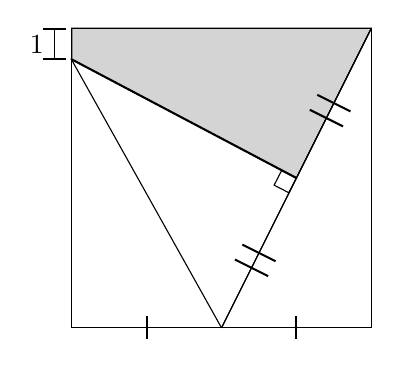
\begin{tikzpicture}[x=0.75pt,y=0.75pt,yscale=-1,xscale=1]
%uncomment if require: \path (0,572); %set diagram left start at 0, and has height of 572

%Shape: Polygon [id:ds5650543958578815] 
\draw  [color={rgb, 255:red, 0; green, 0; blue, 0 }  ,draw opacity=1 ][fill={rgb, 255:red, 212; green, 212; blue, 212 }  ,fill opacity=1 ] (243.02,245.18) -- (387.34,245.18) -- (351.26,317.34) -- (242.8,260.07) -- (243.07,259.26) -- cycle ;
%Shape: Rectangle [id:dp6795345054552426] 
\draw   (243.02,245.18) -- (387.34,245.18) -- (387.34,389.5) -- (243.02,389.5) -- cycle ;
%Straight Lines [id:da192908054306685] 
\draw    (387.34,389.5) -- (243.02,389.5) ;
%Straight Lines [id:da8685436559885313] 
\draw    (387.34,245.18) -- (315.18,389.5) ;
%Straight Lines [id:da42661267614407583] 
\draw [line width=0.75]    (351.26,317.34) -- (242.8,260.07) ;
%Shape: Rectangle [id:dp13649351225462447] 
\draw   (344.17,313.7) -- (351.26,317.34) -- (347.62,324.43) -- (340.53,320.79) -- cycle ;
%Straight Lines [id:da3751189931075172] 
\draw    (351.26,317.34) -- (315.18,389.5) ;
\draw [shift={(333.22,353.42)}, rotate = 296.57] [color={rgb, 255:red, 0; green, 0; blue, 0 }  ][line width=0.75]    (0,8.94) -- (0,-8.94)(-8.04,8.94) -- (-8.04,-8.94)   ;
%Straight Lines [id:da23660260364554286] 
\draw    (387.34,245.18) -- (351.26,317.34) ;
\draw [shift={(369.3,281.26)}, rotate = 296.57] [color={rgb, 255:red, 0; green, 0; blue, 0 }  ][line width=0.75]    (0,8.94) -- (0,-8.94)(-8.04,8.94) -- (-8.04,-8.94)   ;
%Straight Lines [id:da7038593183497226] 
\draw    (242.8,260.07) -- (315.18,389.5) ;

%Straight Lines [id:da5829046438230716] 
\draw    (234.88,245.61) -- (234.88,259.83) ;
\draw [shift={(234.88,259.83)}, rotate = 270] [color={rgb, 255:red, 0; green, 0; blue, 0 }  ][line width=0.75]    (0,5.59) -- (0,-5.59)   ;
\draw [shift={(234.88,245.61)}, rotate = 270] [color={rgb, 255:red, 0; green, 0; blue, 0 }  ][line width=0.75]    (0,5.59) -- (0,-5.59)   ;

%Straight Lines [id:da6956801139387325] 
\draw    (243.02,389.5) -- (315.18,389.5) ;
\draw [shift={(279.1,389.5)}, rotate = 180] [color={rgb, 255:red, 0; green, 0; blue, 0 }  ][line width=0.75]    (0,5.59) -- (0,-5.59)   ;
%Straight Lines [id:da00508777911562408] 
\draw    (315.18,389.5) -- (387.34,389.5) ;
\draw [shift={(351.26,389.5)}, rotate = 180] [color={rgb, 255:red, 0; green, 0; blue, 0 }  ][line width=0.75]    (0,5.59) -- (0,-5.59)   ;

% Text Node
\draw (230.73,252.99) node [anchor=east] [inner sep=0.75pt]    {$1$};


\end{tikzpicture}
\end{center}

\fourch{7}{11}{15}{19}

\end{probboxed}

\ans{(d) 19}

\soln 1  Let be the side of the square be $y$ and denote the square as $ABCD$.

\begin{center}
    


\tikzset{every picture/.style={line width=0.75pt}} %set default line width to 0.75pt        

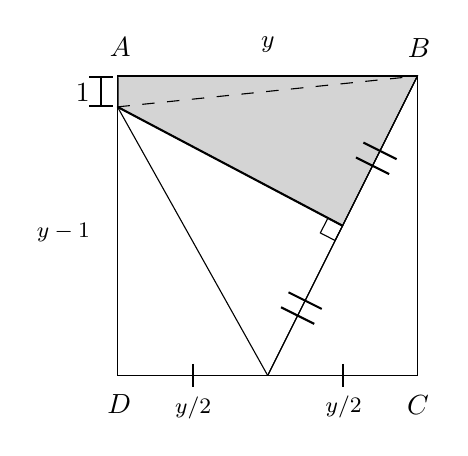
\begin{tikzpicture}[x=0.75pt,y=0.75pt,yscale=-1,xscale=1]
%uncomment if require: \path (0,572); %set diagram left start at 0, and has height of 572

%Shape: Polygon [id:ds016096440841402826] 
\draw  [color={rgb, 255:red, 0; green, 0; blue, 0 }  ,draw opacity=1 ][fill={rgb, 255:red, 212; green, 212; blue, 212 }  ,fill opacity=1 ] (363.22,174.98) -- (507.54,174.98) -- (471.46,247.14) -- (363,189.87) -- (363.27,189.06) -- cycle ;
%Shape: Rectangle [id:dp20973571181245276] 
\draw   (363.22,174.98) -- (507.54,174.98) -- (507.54,319.3) -- (363.22,319.3) -- cycle ;
%Straight Lines [id:da6260868990375161] 
\draw    (507.54,319.3) -- (363.22,319.3) ;
%Straight Lines [id:da6462810265454717] 
\draw    (507.54,174.98) -- (435.38,319.3) ;
%Straight Lines [id:da6148819440812954] 
\draw [line width=0.75]    (471.46,247.14) -- (363,189.87) ;
%Shape: Rectangle [id:dp5514797816132391] 
\draw   (464.37,243.5) -- (471.46,247.14) -- (467.82,254.23) -- (460.73,250.59) -- cycle ;
%Straight Lines [id:da25819615384543915] 
\draw    (471.46,247.14) -- (435.38,319.3) ;
\draw [shift={(453.42,283.22)}, rotate = 296.57] [color={rgb, 255:red, 0; green, 0; blue, 0 }  ][line width=0.75]    (0,8.94) -- (0,-8.94)(-8.04,8.94) -- (-8.04,-8.94)   ;
%Straight Lines [id:da32060892747524483] 
\draw    (507.54,174.98) -- (471.46,247.14) ;
\draw [shift={(489.5,211.06)}, rotate = 296.57] [color={rgb, 255:red, 0; green, 0; blue, 0 }  ][line width=0.75]    (0,8.94) -- (0,-8.94)(-8.04,8.94) -- (-8.04,-8.94)   ;
%Straight Lines [id:da1818033747857437] 
\draw    (363,189.87) -- (435.38,319.3) ;

%Straight Lines [id:da12212269187619818] 
\draw    (355.08,175.41) -- (355.08,189.63) ;
\draw [shift={(355.08,189.63)}, rotate = 270] [color={rgb, 255:red, 0; green, 0; blue, 0 }  ][line width=0.75]    (0,5.59) -- (0,-5.59)   ;
\draw [shift={(355.08,175.41)}, rotate = 270] [color={rgb, 255:red, 0; green, 0; blue, 0 }  ][line width=0.75]    (0,5.59) -- (0,-5.59)   ;

%Straight Lines [id:da626888561042642] 
\draw    (363.22,319.3) -- (435.38,319.3) ;
\draw [shift={(399.3,319.3)}, rotate = 180] [color={rgb, 255:red, 0; green, 0; blue, 0 }  ][line width=0.75]    (0,5.59) -- (0,-5.59)   ;
%Straight Lines [id:da5576986020668606] 
\draw    (435.38,319.3) -- (507.54,319.3) ;
\draw [shift={(471.46,319.3)}, rotate = 180] [color={rgb, 255:red, 0; green, 0; blue, 0 }  ][line width=0.75]    (0,5.59) -- (0,-5.59)   ;
%Straight Lines [id:da34983653351482613] 
\draw  [dash pattern={on 4.5pt off 4.5pt}]  (363,189.87) -- (507.54,174.98) ;

% Text Node
\draw (435.43,159.9) node  [font=\small]  {$y$};
% Text Node
\draw (336.93,250.4) node  [font=\footnotesize]  {$y-1$};
% Text Node
\draw (399.43,334.9) node  [font=\footnotesize]  {$y/2$};
% Text Node
\draw (471.93,334.4) node  [font=\footnotesize]  {$y/2$};
% Text Node
\draw (364.29,161.1) node    {$A$};
% Text Node
\draw (508.29,161.6) node    {$B$};
% Text Node
\draw (507.79,333.6) node    {$C$};
% Text Node
\draw (363.79,333.1) node    {$D$};
% Text Node
\draw (350.93,182.79) node [anchor=east] [inner sep=0.75pt]    {$1$};


\end{tikzpicture}
\end{center}

Let be $E$ one endpoint of a segment with a length of 1 from $A$ and let $F$ be the midpoint of $DC$.

\begin{center}
    


\tikzset{every picture/.style={line width=0.75pt}} %set default line width to 0.75pt        

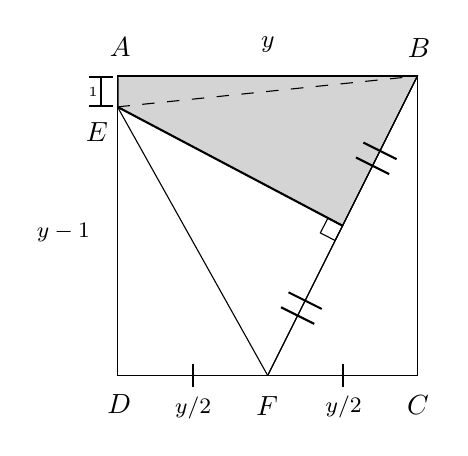
\begin{tikzpicture}[x=0.75pt,y=0.75pt,yscale=-1,xscale=1]
%uncomment if require: \path (0,572); %set diagram left start at 0, and has height of 572

%Shape: Polygon [id:ds016096440841402826] 
\draw  [color={rgb, 255:red, 0; green, 0; blue, 0 }  ,draw opacity=1 ][fill={rgb, 255:red, 212; green, 212; blue, 212 }  ,fill opacity=1 ] (363.22,174.98) -- (507.54,174.98) -- (471.46,247.14) -- (363,189.87) -- (363.27,189.06) -- cycle ;
%Shape: Rectangle [id:dp20973571181245276] 
\draw   (363.22,174.98) -- (507.54,174.98) -- (507.54,319.3) -- (363.22,319.3) -- cycle ;
%Straight Lines [id:da6260868990375161] 
\draw    (507.54,319.3) -- (363.22,319.3) ;
%Straight Lines [id:da6462810265454717] 
\draw    (507.54,174.98) -- (435.38,319.3) ;
%Straight Lines [id:da6148819440812954] 
\draw [line width=0.75]    (471.46,247.14) -- (363,189.87) ;
%Shape: Rectangle [id:dp5514797816132391] 
\draw   (464.37,243.5) -- (471.46,247.14) -- (467.82,254.23) -- (460.73,250.59) -- cycle ;
%Straight Lines [id:da25819615384543915] 
\draw    (471.46,247.14) -- (435.38,319.3) ;
\draw [shift={(453.42,283.22)}, rotate = 296.57] [color={rgb, 255:red, 0; green, 0; blue, 0 }  ][line width=0.75]    (0,8.94) -- (0,-8.94)(-8.04,8.94) -- (-8.04,-8.94)   ;
%Straight Lines [id:da32060892747524483] 
\draw    (507.54,174.98) -- (471.46,247.14) ;
\draw [shift={(489.5,211.06)}, rotate = 296.57] [color={rgb, 255:red, 0; green, 0; blue, 0 }  ][line width=0.75]    (0,8.94) -- (0,-8.94)(-8.04,8.94) -- (-8.04,-8.94)   ;
%Straight Lines [id:da1818033747857437] 
\draw    (363,189.87) -- (435.38,319.3) ;

%Straight Lines [id:da17795935138174035] 
\draw    (355.08,175.41) -- (355.08,189.63) ;
\draw [shift={(355.08,189.63)}, rotate = 270] [color={rgb, 255:red, 0; green, 0; blue, 0 }  ][line width=0.75]    (0,5.59) -- (0,-5.59)   ;
\draw [shift={(355.08,175.41)}, rotate = 270] [color={rgb, 255:red, 0; green, 0; blue, 0 }  ][line width=0.75]    (0,5.59) -- (0,-5.59)   ;
%Straight Lines [id:da626888561042642] 
\draw    (363.22,319.3) -- (435.38,319.3) ;
\draw [shift={(399.3,319.3)}, rotate = 180] [color={rgb, 255:red, 0; green, 0; blue, 0 }  ][line width=0.75]    (0,5.59) -- (0,-5.59)   ;
%Straight Lines [id:da5576986020668606] 
\draw    (435.38,319.3) -- (507.54,319.3) ;
\draw [shift={(471.46,319.3)}, rotate = 180] [color={rgb, 255:red, 0; green, 0; blue, 0 }  ][line width=0.75]    (0,5.59) -- (0,-5.59)   ;
%Straight Lines [id:da34983653351482613] 
\draw  [dash pattern={on 4.5pt off 4.5pt}]  (363,189.87) -- (507.54,174.98) ;

% Text Node
\draw (435.43,159.9) node  [font=\small]  {$y$};
% Text Node
\draw (336.93,250.4) node  [font=\footnotesize]  {$y-1$};
% Text Node
\draw (399.43,334.9) node  [font=\footnotesize]  {$y/2$};
% Text Node
\draw (471.93,334.4) node  [font=\footnotesize]  {$y/2$};
% Text Node
\draw (364.29,161.1) node    {$A$};
% Text Node
\draw (508.29,161.6) node    {$B$};
% Text Node
\draw (507.79,333.6) node    {$C$};
% Text Node
\draw (363.79,333.1) node    {$D$};
% Text Node
\draw (353.13,202.1) node    {$E$};
% Text Node
\draw (351.21,182.79) node  [font=\tiny]  {$1$};
% Text Node
\draw (435.13,334.1) node    {$F$};


\end{tikzpicture}
\end{center}

Next, note that $EF$ is the hypotenuse of $\Delta ADF$ and its adjacent right triangle. And we know from the figure that this right triangle is congruent with the right triangle that has hypotenuse $EB$ (not $\Delta AEB$) because their heights and their bases are congruent. This means $EF = EB.$ This meas $$\dfrac{5y^2}{4} -2y + 1 = y^2 + 1 \Leftrightarrow \dfrac{1}{4}y = 2 \implies y=8$$

This implies $EF=EB=\sqrt{65}$ and $BF = 4\sqrt{5}$. Moreover, the altitude from $E$ to $BF$ is $\sqrt{65-20} = 3\sqrt{5}$. Note that the area of the shaded area is the sum of the areas of the right triangle with side $EB$ and of $\Delta ABE$. Finding area of the right triangle with side $EB$, we have $\dfrac{1}{2}(3\sqrt{5})(2\sqrt{5}) = 15$. Finally for the area of $\Delta ABE$, we have $\dfrac{1}{2}(8)(1) = 4.$

Therefore, the shaded area is \fbox{$15 + 4 = 19$.}

\soln2

For this approach, we are going to use the Cartesian plane. 

\begin{center}
    


\tikzset{every picture/.style={line width=0.75pt}} %set default line width to 0.75pt        

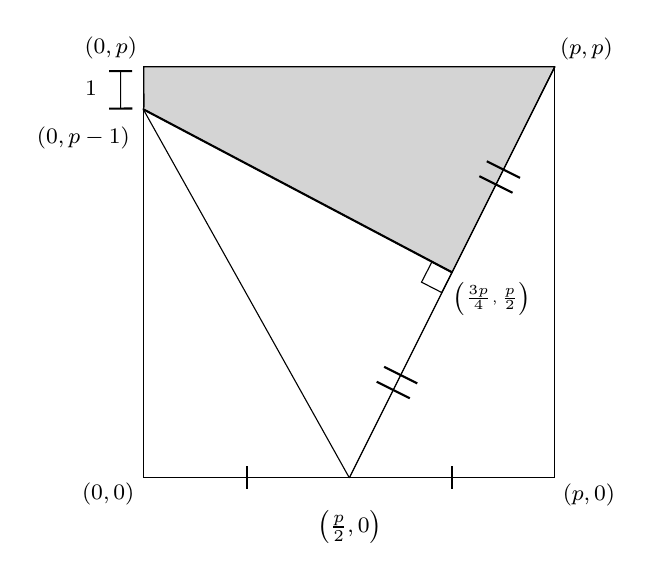
\begin{tikzpicture}[x=0.75pt,y=0.75pt,yscale=-1,xscale=1]
%uncomment if require: \path (0,772); %set diagram left start at 0, and has height of 772

%Shape: Polygon [id:ds2711936305675131] 
\draw  [color={rgb, 255:red, 0; green, 0; blue, 0 }  ,draw opacity=1 ][fill={rgb, 255:red, 212; green, 212; blue, 212 }  ,fill opacity=1 ] (138.51,403.49) -- (336.52,403.49) -- (287.02,502.5) -- (138.22,423.91) -- (138.59,422.81) -- cycle ;
%Shape: Rectangle [id:dp5123222896562338] 
\draw   (138.51,403.49) -- (336.52,403.49) -- (336.52,601.5) -- (138.51,601.5) -- cycle ;
%Straight Lines [id:da12080059603582849] 
\draw    (336.52,601.5) -- (138.51,601.5) ;
%Straight Lines [id:da9352428254916845] 
\draw    (336.52,403.49) -- (237.52,601.5) ;
%Straight Lines [id:da4666561516758394] 
\draw [line width=0.75]    (287.02,502.5) -- (138.22,423.91) ;
%Shape: Rectangle [id:dp2619287795811991] 
\draw   (277.29,497.5) -- (287.02,502.5) -- (282.02,512.22) -- (272.3,507.23) -- cycle ;
%Straight Lines [id:da8893354944018712] 
\draw    (287.02,502.5) -- (237.52,601.5) ;
\draw [shift={(262.27,552)}, rotate = 296.57] [color={rgb, 255:red, 0; green, 0; blue, 0 }  ][line width=0.75]    (0,8.94) -- (0,-8.94)(-8.04,8.94) -- (-8.04,-8.94)   ;
%Straight Lines [id:da7294676425381841] 
\draw    (336.52,403.49) -- (287.02,502.5) ;
\draw [shift={(311.77,452.99)}, rotate = 296.57] [color={rgb, 255:red, 0; green, 0; blue, 0 }  ][line width=0.75]    (0,8.94) -- (0,-8.94)(-8.04,8.94) -- (-8.04,-8.94)   ;
%Straight Lines [id:da8070201387416351] 
\draw    (138.22,423.91) -- (237.52,601.5) ;

%Straight Lines [id:da6622517497078884] 
\draw    (127.32,405.56) -- (127.35,423.58) ;
\draw [shift={(127.35,423.58)}, rotate = 269.92] [color={rgb, 255:red, 0; green, 0; blue, 0 }  ][line width=0.75]    (0,5.59) -- (0,-5.59)   ;
\draw [shift={(127.32,405.56)}, rotate = 269.92] [color={rgb, 255:red, 0; green, 0; blue, 0 }  ][line width=0.75]    (0,5.59) -- (0,-5.59)   ;
%Straight Lines [id:da3844693012723386] 
\draw    (138.51,601.5) -- (237.52,601.5) ;
\draw [shift={(188.01,601.5)}, rotate = 180] [color={rgb, 255:red, 0; green, 0; blue, 0 }  ][line width=0.75]    (0,5.59) -- (0,-5.59)   ;
%Straight Lines [id:da20789125441127299] 
\draw    (237.52,601.5) -- (336.52,601.5) ;
\draw [shift={(287.02,601.5)}, rotate = 180] [color={rgb, 255:red, 0; green, 0; blue, 0 }  ][line width=0.75]    (0,5.59) -- (0,-5.59)   ;

% Text Node
\draw (113.11,413.65) node  [font=\footnotesize]  {$1$};
% Text Node
\draw (121.36,609.16) node  [font=\footnotesize]  {$( 0,0)$};
% Text Node
\draw (122.56,394.4) node  [font=\footnotesize]  {$( 0,p)$};
% Text Node
\draw (351.76,394.8) node  [font=\footnotesize]  {$( p,p)$};
% Text Node
\draw (109.36,437.6) node  [font=\footnotesize]  {$( 0,p-1)$};
% Text Node
\draw (352.96,610) node  [font=\footnotesize]  {$( p,0)$};
% Text Node
\draw (237.76,625.2) node  [font=\footnotesize]  {$\left(\frac{p}{2} ,0\right)$};
% Text Node
\draw (306.16,515.2) node  [font=\tiny]  {$\left(\frac{3p}{4} ,\frac{p}{2}\right)$};


\end{tikzpicture}
\end{center}

Note that the distance between $(0,p-1)$ and $(\frac{p}{2}, 0)$ and the distance between $(0,p-1)$ and $(p,p)$ are equal. Finding $p$, we have $p=8$. 

Now, we can invoke the Shoelace theorem using the coordinates $(0,8), (8,8), (0,7), (6,4)$ to find the shaded area $A$! 


\begin{equation*}
  \begin{array}{lll}
    A & = & \dfrac{1}{2} 	\big |  (8\cdot8 + 0\cdot7 + 0\cdot4 + 6\cdot8)-(8\cdot4 + 6\cdot7 + 0\cdot8 + 0\cdot8) \big |    \\
    
    \\
    
    A & = & \dfrac{1}{2} 	\big | (112)-(74) 	\big |    \\
    
    \\
    
    A & = & \dfrac{1}{2} 	\big | 38 \big |  = 19   \\
     
  \end{array}
\end{equation*}


Hence, our shaded area is equal to \fbox{19}.

\begin{mdframed}
\begin{rem}
The approach of \textbf{Solution 2} can be applied to \href{https://pmo.ph/wp-content/uploads/2021/02/PMO23-Qualifying-Round.pdf}{PMO 23 Qualifying I.9}: 

"Point $G$ lies on side $AB$ of square $ABCD$ and square $AEFG$is drawn outwards $ABCD$, as
shown in the figure below. Suppose that the area of triangle $EGC$ is $1/16$ of the area of
pentagon $DEFBC$. What is the ratio of the areas of $AEFG$ and $ABCD$?"

\end{rem}

\begin{rem} Also, this problem is similar to \href{https://pmo.ph/wp-content/uploads/2019/11/PMO-22-Qualifying-Round-with-answers.pdf}{PMO 22 Qualifying I.12}:

"The figure below shows a parallelogram $ABCD$ with $CD = 18$. Point F lies inside $ABCD$ and
lines $AB$ and $DF$ meet at $E$. If $AE = 12$ and the areas of triangles $FEB$ and $FCD$ are 30
and $162$, respectively, find the area of triangle $BFC$."
\end{rem}
\end{mdframed}

\subsubsection{Item \# 14}

\begin{probboxed}
\item Bryce plays a game in which he flips a fair coin repeatedly. In each flip, he obtains two tokens if the coin lands on heads, and loses one coin if it's tails. From the beginning, he has nine tokens. If after nine flips, he still retains the number of tokens he had from the beginning. Find the probability of Bryce having nine tokens at the end. 

\fourch{1/7}{1/6}{5/28}{17/84}
\end{probboxed}

\ans{(a) 1/7}

\sol Let $n$ be the number that Bryce win such that $9 + \left(2n-(9-n)\right) = 9 $. Finding $n$ gives us 3. This means, Bryce won 3 times and lose 6 times. Next, let $W$ represent his win and $L$ for his loss such that we have 3$W$s and 6$L$s. If we are going to make a permutation out of these letters, we have $\dbinom{9}{6} = 84$ total ways to do so.

Next, consider the following permutation: $$W * W * W*$$ Our goal here is to find the number of permutations with these conditions, and these are:

\begin{itemize}
    \item For the first $*$, you can only have $m \leq 2 L$'s. (In this case, denote this as $a = a' + m - 2.$)
    \item In the second $*$, you can then have at most $(4 - m) L$'s. (In this case, denote this as $b = b' + m - 4.$)
    \item In the last $*$, you can have all the remaining $L$'s. (In this case, denote this as $c = 6 - m.$)
  
     \end{itemize}
     
   Adding all of them gives us $a' + b ' + m = 6$. Since $m \leq 2$, let us have some cases to calculate the number of ways to accomplish our goal using Stars and bars or Balls and urns
   
   \begin{itemize}
       \item If $m=0$, we have $\dbinom{6-1}{2-1} = \dbinom{5}{1} = 5$ ways.
       
       \item If $m=1$, we have $\dbinom{5-1}{2-1} = \dbinom{4}{1} = 4$ ways.
       
       \item If $m=2$, we have $\dbinom{4-1}{2-1} = \dbinom{3}{1} = 3$ ways.
   \end{itemize}
   
   Hence, we have $5+4+3 = 12$ ways to accomplish our goal. Finding the probability to accomplish this gives us $\dfrac{12}{84} = \dfrac{1}{7}$. Hence, our final answer is \fbox{(d) $1/7$}.


\subsubsection{Item \# 15}

\begin{probboxed}
How many ways are there to arrange the first ten positive integers such that the multiples of 2 appear in increasing order, and the multiples of 3 appear in decreasing order?

\fourch{720}{2160}{5040}{6480}
\end{probboxed}

\ans{(d) 6480}

\sol

Note that if we are going to arrange the sequence, we have $$ 1, 2, 9, 4, 5, 6, 7, 8, 3, 10 $$. But for the sake of generality, let us make the sequence like this:

$$ *, 2, *, 4, *, 6, *, 8, *, 10 $$ where $*$ is an empty urn that can be occupied by a number from set $N \in \{1,5,7,3,9\}$. W are going to focus first on the multiples of 3. Note that $9$ must be first before $3$ to satisfy the problem condition. For $9$ to be arranged in the sequence, we have 3 ways for this to be accomplished. Same for $3$, we have 3 ways for this as well. 

For numbers $1,5,7$, we have $\dbinom{3+8-1}{8-1} = \dbinom{10}{7}$ to arrange these numbers. And we have $3!$ to arrange in their set: $(3,5,7)$. 

Hence, we have $3 \cdot 3 \cdot \dbinom{10}{7} \cdot 3! = \fbox{6480}$ ways as our final answer.

\begin{mdframed}
\begin{rem}
The solution is from Dumplet's video: \url{https://www.youtube.com/watch?v=eTKpoLpV9ZU}.
\end{rem}
\end{mdframed}

\newpage

\subsection{PART II}

All answers are positive integers. Do not use commas if there are more than 3 digits, e,g., type 1234 instead of 1,234. A fraction $a/b$ is in lowest terms if $a$ and $b$ are positive integers whose greatest common factor is 1. Each correct answer is worth five points. 

\subsubsection{Item \# 16}

\begin{probboxed}
What is the largest multiple of 7 less than 10,000 which can be expressed as the sum of squares of three consecutive numbers?
\end{probboxed}

\ans{8750}

\soln1 

Consider the following: $$(n-1)^2 + n^2 + (n+1)^2 \equiv 0 \pmod{7}.$$ Expanding the terms gives us $3n^2 \equiv -2 \pmod{7}$. Multiplying it by 5 gives us $n^2 \equiv 25 \pmod{7}$. Now, we are dealing with 2 cases that $n \equiv -5 \pmod{7}$ or $n \equiv 5 \pmod{7}$.


Because we are dealing with two cases, let us have the following:

\begin{itemize}
    \item If $n \equiv -5 \pmod{7}$, then we have $n \equiv 2, 9, ... , 58$.
    
    \item If $n \equiv 5 \pmod{7}$, then we have $n \equiv 12,19, ... , 54$.
\end{itemize}

If we are going to use the first case, $n=51$ is too small while $n = 58$ is more than 10,000. If we are going to use the second case, we see that $n = 54$ satisfies the condition.

Substituting $n$ with 54 in the original equation gives us \fbox{$8750$}.

\soln2

Trial and error may do if you consider the following function: $$(n-1)^2 + n^2 + (n+1)^2 \equiv 0 \pmod{7}.$$ Just start from $60$ and you get that $n = 54$.

\soln3

Let's express our consecutive squares as $(n-1)^2$, $n^2$, $(n+1)^2$. $(n-1)^2 + n^2 + (n+1)^2 = 3n^2 + 2$. We need $3n^2 + 2 < 10000$, so $n^2 < 3333$, and therefore $n < 58$.

We want to find when $3n^2 + 2 \equiv 0 {\ (\mathrm{mod}\ 7)}$. It's clear that this is only the case when $n^2 \equiv 4 {\ (\mathrm{mod}\ 7)}$, and therefore $n \equiv 2, 5 {\ (\mathrm{mod}\ 7)}$.

From here we just need to find the greatest integer $n$ less than $58$ that is $2, 5 {\ (\mathrm{mod}\ 7)}$, which is $n = 54$. From here we have $53^2 + 54^2 + 55^2 = \boxed{8750}$, our greatest multiple of 7.

\begin{mdframed}
\begin{rem}
With special thanks to \href{https://artofproblemsolving.com/community/user/536265}{CosmoMonkhouse} for Solution 3.
\end{rem}
\end{mdframed}
\subsubsection{Item \# 17}

\begin{probboxed}
Suppose that the polynomial $P(x) = x^3 + 4x^2 + bx +c$ has a single root $r$ and a double root $s$ for some distinct real numbers $r$ and $s$. Given that $P(-2s) = 324$, what is the sum of all possible values of $|c|$?
\end{probboxed}


\ans{108}

\soln1

By Vieta's formulas, $r+2s = -4, s(s + 2r) = b$ and $rs^2 = -c$. Note that $P(-2s) = -8s^3 + 16s^2 -2bs + c = 324$. Substituting $c$ with $-rs^2$ in $P(-2s)$ gives us $$ -8s^3 + 16s^2 -2bs + c = 324 \Leftrightarrow s\left(-8s^2 + 16s -2b -rs\right) = 324.$$ Substitute $2b$ with $2s(s+2r)$ and we have: $$s\left(-8s^2 + 16s -2s(s+2r) -rs\right) \implies s^2\left(-8s + 16 -2(s+2r) -r\right) = 324 $$

Simplifying the expression gives us the following: $$\implies s^2\left(16 -5(r+2s)\right) = s^2 = 9 \implies s = \pm 3$$. Now, we deal with two cases when $s=3$ or $s=-3$. In this way, we can finally solve for the values of $|c|$!


\begin{itemize}
    \item If $s=3$, then $r=-10$. Hence $|c| = |-10\cdot(3)^2| = 90.$
    \item If $s=-3$, then $r=2$. Hence $|c| = |2\cdot(-3)^2| = 18.$
\end{itemize}

Adding the possible values of $|c|$ gives us $90+18 = \fbox{108}$. 

\soln2

By Vieta's formulas, consider the following system:

\begin{center}
    \begin{cases} r+2s = -4 \\ 2rs + s^2 =b \\ rs^2 = -c \end{cases}
    
\end{center}
Note that $P(x) = (x-r)(x-s)^2$, $(2s+4)s^2 = c$ and $P(-2s) = (-2s-r)(-3s^2) = 324.$ Going onto the process will give you the same results. 


\begin{mdframed}
\begin{rem}
Basically, the problem is just algebraic manipulation. Speaking of that, you can watch the latest PMO tutorial video from YouTube titled \href{https://www.youtube.com/watch?v=AZbRengyDs4&t=227s}{[PMO Tutorial #11] Algebraic Manipulation - Algebra}. In that video, try to solve some problems being presented there. It is fun! 
\end{rem}

\begin{rem}
Solution 2 comes from \textbf{Charles Dwight Pelaez} and from \textbf{Benedict Rodil.} Thanks to these people.
\end{rem}
\end{mdframed}



\subsubsection{Item \# 18}

\begin{probboxed}
 Let $m$ and $n$ be relatively prime positive integers. If $m^3n^5$ has 209 positive divisors, then how many positive divisors does $m^5n^3$ have?
\end{probboxed}
\ans{217}

\soln1

Let $m$ be $p^{r_1r_2...r_k}$ and $n$ be $q^{w_1w_2...w_j}$. This implies that $209 = \left(3(r_1r_2...r_k) + 1\right)\left(5(r_1r_2...r_k) + 1\right)$. This implies $(r_1r_2...r_k) = 6$ and $(r_1r_2...r_k) =2$. Now, we got the values of these exponents, we have $m^5n^3 = (p^6)^5 (p^2)^3$. Finding the sum of its positive divisors gives us $(30+1)(6+1) = \fbox{217}$. Hence we got the final answer

\soln2

$209$ factors as $11\cdot19$ so therefore $m^3$ and $n^5$ are $18$th and $10$th powers of a prime, respectively (since $0$ and $208$ aren't divisible by $3$ and $5$ and note that they must each be a power of a single prime since $11$ and $19$ are prime). Thus $n$ is the prime of a square and $m$ is a prime to the $6$th power. Thus $n^3$ is a prime raised to the $6$th power and $m^5$ is an number raised to the $30$th power, so the product has $(6+1)(30+1)=7*31=217$ factors.

\begin{mdframed}
\begin{rem}
Actually, you can let $m$ and $n$ be the products of many primes with different exponents but either way, you can get the same result. For my case, I just made my solution more "narrow" because the goal here overall is to find the sum of the positive divisors not the values of $m$ and $n$.
\end{rem}

\begin{rem}
Special thanks to \href{https://artofproblemsolving.com/community/user/470584}{Sleepy Head of AoPS} for \joshbf{Solution 2}.
\end{rem}
\end{mdframed}

\subsubsection{Item \# 19}

\begin{probboxed}
Let $x$ be a positive real number. What is the maximum value of $\dfrac{2022x^2 \log(x+2022)}{\left(\log(x+2022)\right)^3 + 2x^3}$?
\end{probboxed}

\ans {$674$}

\soln1  Let $a = \left(\log(x+2022)\right)^$. "Flip-flop" the numerator and the denominator and we have $$\dfrac{a^3}{2022x^2(a)} + \dfrac{2x^3}{2022x^2(a)}.$$ In this case, we are asked to find the minimum instead. By trivial inequality, we have $$ \dfrac{1}{2022} \left(\dfrac{a^3}{x^2(a)} + \dfrac{2x^3}{x^2(a)} \right) \geq \dfrac{1}{2022} \left(\frac{3x^3}{x^3}\right) = \dfrac{3}{2022}.$$ Such inequality can be achieved iff. $a = x$. Hence, $$ L.H.S \geq \dfrac{1}{674}.$$ But since this is the minimum of the transformed expression, the inverse of it must be the maximum, Hence our answer is \fbox{$674$}.

\soln2

Another approach is a direct application of GM-AM Inequality. Since the expression is not a radical then we can safely assume that $$\sqrt{\left(\dfrac{2022x^2 \log(x+2022)}{\left(\log(x+2022)\right)^3 + 2x^3}\right)^2} \leq \dfrac{\dfrac{2022x^2 \log(x+2022)}{\left(\log(x+2022)\right)^3 + 2x^3} + \dfrac{2022x^2 \log(x+2022)}{\left(\log(x+2022)\right)^3 + 2x^3}}{2}.$$ Note that such inequality can be achieved when $\log(x+2022) = x$. As a result, we have $$\dfrac{2022x^2 \log(x+2022)}{\left(\log(x+2022)\right)^3 + 2x^3} = \sqrt{\left(\dfrac{2022x^2 \log(x+2022)}{\left(\log(x+2022)\right)^3 + 2x^3}\right)^2} \leq \dfrac{1348}{2} = 674.$$

Hence, we got the same answer.

\begin{mdframed}
\begin{rem}
This problem reminds me of a 2019 PMO question which is from \href{https://pmo.ph/wp-content/uploads/2019/11/PMO-22-Qualifying-Round-with-answers.pdf}{PMO 22 Qualifying III.5}. The problem states that

"Find the minimum value of $$\dfrac{7x^2 -2xy + 3y^2}{x^2 -y^2}$$ if $x$ and $y$ are positive real numbers such that $x > y$."


\end{rem}

\begin{rem}
This problem also reminds me of a PMO problem from \href{http://pmo.ph/wp-content/uploads/2018/08/PMO-20-Qualifying-Round-with-answers-only.pdf}{PMO 20 Qualifying III.3}.

"Find the minimum value of $$\dfrac{18}{a+b}+\dfrac{12}{ab}+8a+5b,$$ where $a$ and $b$ are positive real numbers.
\end{rem}
\end{mdframed}

\newpage

\subsubsection{Item \# 20}

\begin{probboxed}
Let $a,b,c$ be real numbers such that $$3ab + 2 = 6b, \quad 3bc + 2 = 5c, \quad 3ca + 2 =4a.$$
    
   Suppose the only possible values for the product $abc$ are $r/s$ and $t/u$, where $r/s $ and $t/u$ are both fractions in lowest terms. Find $r+s+t+u.$
\end{probboxed}

\ans{18}

\sol

Multiply all equations give us this form: $$27a^2b^2c^2 + 18a^2bc +18ab^2 + 18abc^2 + 12ab + 12bc + 12ac + 8 =120abc$$. Factoring gives us this:

\vspace{-1cm}

\begin{center}
    \begin{equation*}
        \begin{array}{llll}
            \implies & 27a^2b^2c^2 + 18a^2bc +18ab^2c + 18abc^2 + 12ab + 12bc + 12ac + 8 & = & 120abc \\
            
           \implies & \hspace{7mm} 27a^2b^2c^2 + 6ac(3ab +2) + 6ab(3bc+2) + 6bc(3ca +2) + 8 & = & 120abc \\
           
           \implies &  \hspace{7cm} 27a^2b^2c^2 + 90abc + 8 & = & 120abc \\
           
           \implies &  \hspace{7cm}  (9abc -4) (3abc -2) & = & 0\\
        \end{array}
    \end{equation*}
\end{center}

This gives us $abc= \frac{4}{9}, \frac{2}{3} $  Hence, $r+t+s+u = 4 + 9 + 2 + 3 = \fbox{18}$.



\begin{mdframed}
\begin{rem}
I would like to thank \textbf{Charles Dwight Pelaez} for giving me this solution.
\end{rem}

\begin{rem}
Try this problem from \joshbf{Purple Comet 2016 High School}:

"Positive integers a, b, c, d, and e satisfy the equations



\begin{center}
    \begin{cases} (a + 1)(3bc + 1) = d + 3e + 1 \\ (b + 1)(3ca + 1) = 3d + e + 13 \\ (c + 1)(3ab + 1) = 4(26-d- e) - 1 \end{cases}
    
\end{center}

Find $d^2+e^2$."
\end{rem}

\begin{rem} Try this problem from \href{https://pmo.ph/wp-content/uploads/2021/01/10th-PMO-Area-National-Stage-Questions-with-Answers.pdf}{PMO 10 Areas I.11}: Solve the system of equations:

\begin{center}
\begin{cases} x + y + \sqrt{xy} = 28 \\ x^2 + y^2 + xy = 28.

\end{cases}
\end{center}

\end{rem}
\end{mdframed}




\subsubsection{Item \# 21}

\begin{probboxed}
You roll a fair 12-sided die repeatedly. The probability that all primes show up at least once before seeing any of the other numbers can be expressed as a fraction $p/q$ in lowest terms. What is $p+q$?
\end{probboxed}

\ans{793}

\sol Choose 5 numbers out from 12 gives us $\dbinom{12}{5}=792$. The probability that we chose all prime numbers gives us $\dbinom{5}{5}=1$. Hence, the probability that all primes show up at least once before seeing any of the other numbers is $\dfrac{1}{792} = \dfrac{p}{q}.$ In conclusion, $p+q=\fbox{793.}$
 
\subsubsection{Item \# 22}

\begin{probboxed}
Let $PMO$ be a triangle with $PM =2$ and $\angle PMO = 120^{\circ}$. Let $B$ be a point on $PO$ such that $PM$ is perpendicular to $MB$ and suppose that $PM=BO$. The product of the lengths of the sides of the triangle can be expressed in the form $a + b\sqrt[3]{c}$, where $a,b,c$ are positive integers and $c$ is minimized. Find $a+b+c$.
\end{probboxed}

\ans{28}

\sol

\begin{center}
    


\tikzset{every picture/.style={line width=0.75pt}} %set default line width to 0.75pt        

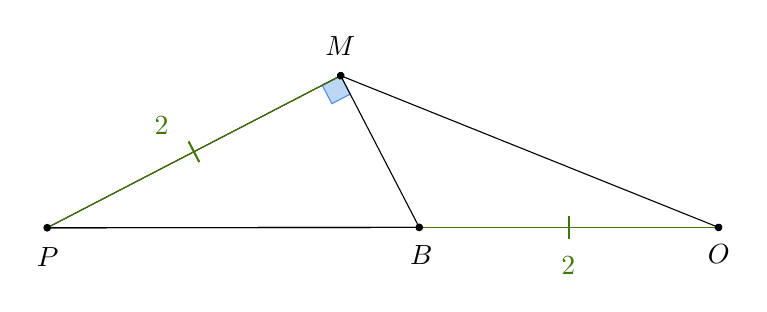
\begin{tikzpicture}[x=0.75pt,y=0.75pt,yscale=-1,xscale=1]
%uncomment if require: \path (0,1128); %set diagram left start at 0, and has height of 1128

%Shape: Rectangle [id:dp09152640714646809] 
\draw  [color={rgb, 255:red, 74; green, 144; blue, 226 }  ,draw opacity=1 ][fill={rgb, 255:red, 74; green, 144; blue, 226 }  ,fill opacity=0.37 ] (198.05,664.03) -- (206.92,659.4) -- (211.55,668.27) -- (202.68,672.9) -- cycle ;
%Shape: Right Triangle [id:dp647890274132146] 
\draw   (244.79,732.49) -- (65.53,732.66) -- (206.92,659.4) -- cycle ;
%Straight Lines [id:da2539304271966736] 
\draw [color={rgb, 255:red, 65; green, 117; blue, 5 }  ,draw opacity=0.99 ]   (65.53,732.66) -- (206.92,659.4) ;
\draw [shift={(136.22,696.03)}, rotate = 152.61] [color={rgb, 255:red, 65; green, 117; blue, 5 }  ,draw opacity=0.99 ][line width=0.75]    (0,5.59) -- (0,-5.59)   ;
%Straight Lines [id:da280545336489908] 
\draw [color={rgb, 255:red, 65; green, 117; blue, 5 }  ,draw opacity=0.99 ]   (244.79,732.49) -- (389,732.49) -- cycle ;
\draw [shift={(316.9,732.49)}, rotate = 180] [color={rgb, 255:red, 65; green, 117; blue, 5 }  ,draw opacity=0.99 ][line width=0.75]    (0,5.59) -- (0,-5.59)   ;
\draw [shift={(316.9,732.49)}, rotate = 360] [color={rgb, 255:red, 65; green, 117; blue, 5 }  ,draw opacity=0.99 ][line width=0.75]    (0,5.59) -- (0,-5.59)   ;
%Straight Lines [id:da48389186181433774] 
\draw    (65.53,732.66) -- (244.79,732.49) ;
\draw [shift={(244.79,732.49)}, rotate = 359.95] [color={rgb, 255:red, 0; green, 0; blue, 0 }  ][fill={rgb, 255:red, 0; green, 0; blue, 0 }  ][line width=0.75]      (0, 0) circle [x radius= 1.34, y radius= 1.34]   ;
\draw [shift={(65.53,732.66)}, rotate = 359.95] [color={rgb, 255:red, 0; green, 0; blue, 0 }  ][fill={rgb, 255:red, 0; green, 0; blue, 0 }  ][line width=0.75]      (0, 0) circle [x radius= 1.34, y radius= 1.34]   ;
%Straight Lines [id:da8667968060220101] 
\draw    (206.92,659.4) -- (389,732.49) ;
\draw [shift={(389,732.49)}, rotate = 21.87] [color={rgb, 255:red, 0; green, 0; blue, 0 }  ][fill={rgb, 255:red, 0; green, 0; blue, 0 }  ][line width=0.75]      (0, 0) circle [x radius= 1.34, y radius= 1.34]   ;
\draw [shift={(206.92,659.4)}, rotate = 21.87] [color={rgb, 255:red, 0; green, 0; blue, 0 }  ][fill={rgb, 255:red, 0; green, 0; blue, 0 }  ][line width=0.75]      (0, 0) circle [x radius= 1.34, y radius= 1.34]   ;

% Text Node
\draw (206.77,645.27) node    {$M$};
% Text Node
\draw (245.77,745.93) node    {$B$};
% Text Node
\draw (65.77,746.93) node    {$P$};
% Text Node
\draw (389.11,745.27) node    {$O$};
% Text Node
\draw (120.56,683.6) node  [color={rgb, 255:red, 65; green, 117; blue, 5 }  ,opacity=0.99 ]  {$2$};
% Text Node
\draw (316.56,750.93) node  [color={rgb, 255:red, 65; green, 117; blue, 5 }  ,opacity=0.99 ]  {$2$};


\end{tikzpicture}
\end{center}

The first thing comes to mind if you are going to talk about the product of the sides oa triangle, we can immediately think of the circumcircle area forumla which states that: $$A = \dfrac{abc}{4R}$$ if $a,b,c$ are the sides of the triangle, $A$ for the area of the triangle and $R$ for the \textbf{circumradius of the triangle.} Since, we are looking for the product of the sides, then $abc = 4AR$. For the sake of avoiding confusion, let the product of the sides of $PMO$ be $N$.



Let $\angle MPO = x$. Then, we have the following figure:

\begin{center}



\tikzset{every picture/.style={line width=0.75pt}} %set default line width to 0.75pt        

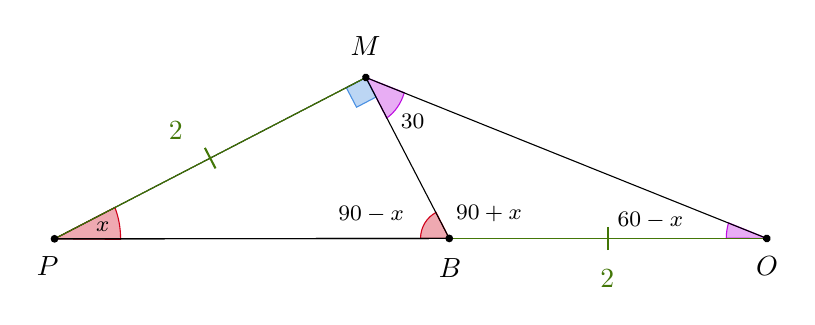
\begin{tikzpicture}[x=0.75pt,y=0.75pt,yscale=-1,xscale=1]
%uncomment if require: \path (0,1465); %set diagram left start at 0, and has height of 1465

%Shape: Pie [id:dp06913736278978] 
\draw  [color={rgb, 255:red, 189; green, 16; blue, 224 }  ,draw opacity=1 ][fill={rgb, 255:red, 189; green, 16; blue, 224 }  ,fill opacity=0.34 ] (387,967.75) .. controls (387.01,965.18) and (387.39,962.71) .. (388.08,960.41) -- (406.52,967.89) -- cycle ;
%Shape: Pie [id:dp5104133616501689] 
\draw  [color={rgb, 255:red, 189; green, 16; blue, 224 }  ,draw opacity=1 ][fill={rgb, 255:red, 189; green, 16; blue, 224 }  ,fill opacity=0.34 ] (231.84,897.69) .. controls (230.34,902.82) and (227.32,907.13) .. (223.4,909.88) -- (213.35,890.35) -- cycle ;
%Shape: Pie [id:dp8809917506594758] 
\draw  [color={rgb, 255:red, 208; green, 2; blue, 27 }  ,draw opacity=1 ][fill={rgb, 255:red, 208; green, 2; blue, 27 }  ,fill opacity=0.34 ] (239.69,967.88) .. controls (239.7,962.45) and (242.72,957.73) .. (247.14,955.38) -- (253.53,967.89) -- cycle ;
%Shape: Pie [id:dp8690988707233842] 
\draw  [color={rgb, 255:red, 208; green, 2; blue, 27 }  ,draw opacity=1 ][fill={rgb, 255:red, 208; green, 2; blue, 27 }  ,fill opacity=0.34 ] (92.44,952.97) .. controls (94.2,957.58) and (95.18,962.69) .. (95.18,968.07) .. controls (95.18,968.15) and (95.18,968.24) .. (95.18,968.32) -- (63.35,968.07) -- cycle ;
%Shape: Rectangle [id:dp9902922820587876] 
\draw  [color={rgb, 255:red, 74; green, 144; blue, 226 }  ,draw opacity=1 ][fill={rgb, 255:red, 74; green, 144; blue, 226 }  ,fill opacity=0.37 ] (203.94,895.27) -- (213.35,890.35) -- (218.27,899.76) -- (208.86,904.68) -- cycle ;
%Shape: Right Triangle [id:dp6287494315968176] 
\draw   (253.53,967.89) -- (63.35,968.07) -- (213.35,890.35) -- cycle ;
%Straight Lines [id:da06236962345639574] 
\draw [color={rgb, 255:red, 65; green, 117; blue, 5 }  ,draw opacity=0.99 ]   (63.35,968.07) -- (213.35,890.35) ;
\draw [shift={(138.35,929.21)}, rotate = 152.61] [color={rgb, 255:red, 65; green, 117; blue, 5 }  ,draw opacity=0.99 ][line width=0.75]    (0,5.59) -- (0,-5.59)   ;
%Straight Lines [id:da5287239739426357] 
\draw [color={rgb, 255:red, 65; green, 117; blue, 5 }  ,draw opacity=0.99 ]   (253.53,967.89) -- (406.52,967.89) -- cycle ;
\draw [shift={(330.03,967.89)}, rotate = 180] [color={rgb, 255:red, 65; green, 117; blue, 5 }  ,draw opacity=0.99 ][line width=0.75]    (0,5.59) -- (0,-5.59)   ;
\draw [shift={(330.03,967.89)}, rotate = 360] [color={rgb, 255:red, 65; green, 117; blue, 5 }  ,draw opacity=0.99 ][line width=0.75]    (0,5.59) -- (0,-5.59)   ;
%Straight Lines [id:da7141254239207411] 
\draw    (63.35,968.07) -- (253.53,967.89) ;
\draw [shift={(253.53,967.89)}, rotate = 359.95] [color={rgb, 255:red, 0; green, 0; blue, 0 }  ][fill={rgb, 255:red, 0; green, 0; blue, 0 }  ][line width=0.75]      (0, 0) circle [x radius= 1.34, y radius= 1.34]   ;
\draw [shift={(63.35,968.07)}, rotate = 359.95] [color={rgb, 255:red, 0; green, 0; blue, 0 }  ][fill={rgb, 255:red, 0; green, 0; blue, 0 }  ][line width=0.75]      (0, 0) circle [x radius= 1.34, y radius= 1.34]   ;
%Straight Lines [id:da26691311126144623] 
\draw    (213.35,890.35) -- (406.52,967.89) ;
\draw [shift={(406.52,967.89)}, rotate = 21.87] [color={rgb, 255:red, 0; green, 0; blue, 0 }  ][fill={rgb, 255:red, 0; green, 0; blue, 0 }  ][line width=0.75]      (0, 0) circle [x radius= 1.34, y radius= 1.34]   ;
\draw [shift={(213.35,890.35)}, rotate = 21.87] [color={rgb, 255:red, 0; green, 0; blue, 0 }  ][fill={rgb, 255:red, 0; green, 0; blue, 0 }  ][line width=0.75]      (0, 0) circle [x radius= 1.34, y radius= 1.34]   ;

% Text Node
\draw (213.2,875.36) node    {$M$};
% Text Node
\draw (253.87,982.15) node    {$B$};
% Text Node
\draw (60.06,981.17) node    {$P$};
% Text Node
\draw (406.63,981.44) node    {$O$};
% Text Node
\draw (121.74,916.02) node  [color={rgb, 255:red, 65; green, 117; blue, 5 }  ,opacity=0.99 ]  {$2$};
% Text Node
\draw (329.67,987.46) node  [color={rgb, 255:red, 65; green, 117; blue, 5 }  ,opacity=0.99 ]  {$2$};
% Text Node
\draw (86.64,962.45) node  [font=\footnotesize]  {$x$};
% Text Node
\draw (215.84,956.44) node  [font=\footnotesize]  {$90-x$};
% Text Node
\draw (235.88,911.37) node  [font=\footnotesize]  {$30$};
% Text Node
\draw (272.67,956.13) node  [font=\footnotesize]  {$90+x$};
% Text Node
\draw (350.42,959.18) node  [font=\footnotesize]  {$60-x$};


\end{tikzpicture}
\end{center}

You can obtain these values by angle chasing. Next, note that by trigonometric functions, $PB = \dfrac{2}{\cos x}$. Now, to find the circumradius $R$, recall that by extended law of sines, $2R = \dfrac{a}{\sin \theta}$ for some $\theta$ and $a$. Since we have $\angle PMO = 120^{\circ}$, we have $R = \dfrac{2\sqrt{3}}{3} \left(1 + \dfrac{1}{\cos x}\right)$. Now, we shall find the area $A$ by the fact that $A = \dfrac{1}{2}mn \sin \omega$ (for some side lengths $m$ and $n$, forming the angle $\omega$.) You may think that you may go for the area in terms of the angle $PMO$ but we do not know what is $MO$ yet. So, we will go for $\angle MPO$, and as a result, we have $$A = \dfrac{1}{2}(2)\left(\dfrac{2}{\cos x} \right) \sin x \implies 2\tan x + 2\sin x.$$

 Going back to $abc,$ as we already find the necessary information, we have: $$abc = 4(2\tan x + 2\sin x)\left(\dfrac{2\sqrt{3}}{3} \left(1 + \dfrac{1}{\cos x}\right)\right)$$

\begin{center}



\tikzset{every picture/.style={line width=0.75pt}} %set default line width to 0.75pt        

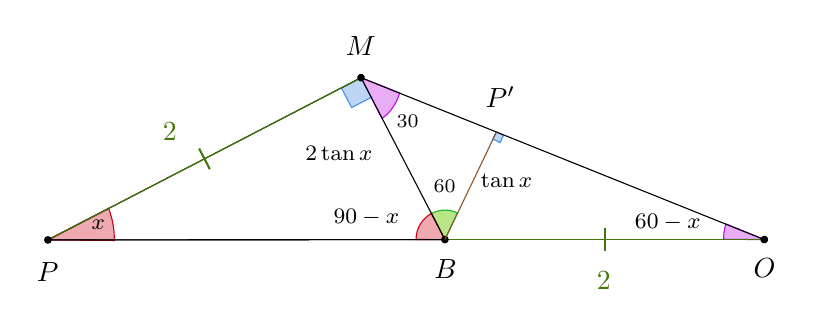
\begin{tikzpicture}[x=0.75pt,y=0.75pt,yscale=-1,xscale=1]
%uncomment if require: \path (0,1465); %set diagram left start at 0, and has height of 1465

%Shape: Pie [id:dp7953886913613673] 
\draw  [color={rgb, 255:red, 27; green, 185; blue, 41 }  ,draw opacity=1 ][fill={rgb, 255:red, 126; green, 211; blue, 33 }  ,fill opacity=0.54 ] (258.76,1138.35) .. controls (260.69,1137.31) and (262.89,1136.73) .. (265.22,1136.73) .. controls (267.36,1136.73) and (269.38,1137.22) .. (271.19,1138.1) -- (265.22,1150.92) -- cycle ;
%Shape: Rectangle [id:dp5973862420761931] 
\draw  [color={rgb, 255:red, 74; green, 144; blue, 226 }  ,draw opacity=1 ][fill={rgb, 255:red, 74; green, 144; blue, 226 }  ,fill opacity=0.37 ] (291.77,1104.17) -- (293.46,1100.66) -- (289.95,1098.97) -- (288.26,1102.48) -- cycle ;
%Shape: Pie [id:dp2999705223959257] 
\draw  [color={rgb, 255:red, 189; green, 16; blue, 224 }  ,draw opacity=1 ][fill={rgb, 255:red, 189; green, 16; blue, 224 }  ,fill opacity=0.34 ] (399.46,1150.78) .. controls (399.48,1148.19) and (399.86,1145.71) .. (400.55,1143.39) -- (419.1,1150.92) -- cycle ;
%Shape: Pie [id:dp7436354786801254] 
\draw  [color={rgb, 255:red, 189; green, 16; blue, 224 }  ,draw opacity=1 ][fill={rgb, 255:red, 189; green, 16; blue, 224 }  ,fill opacity=0.34 ] (243.4,1080.31) .. controls (241.89,1085.47) and (238.85,1089.8) .. (234.91,1092.57) -- (224.81,1072.92) -- cycle ;
%Shape: Pie [id:dp4466767826506133] 
\draw  [color={rgb, 255:red, 208; green, 2; blue, 27 }  ,draw opacity=1 ][fill={rgb, 255:red, 208; green, 2; blue, 27 }  ,fill opacity=0.34 ] (251.3,1150.9) .. controls (251.31,1145.44) and (254.34,1140.7) .. (258.79,1138.33) -- (265.22,1150.92) -- cycle ;
%Shape: Pie [id:dp24583887444282593] 
\draw  [color={rgb, 255:red, 208; green, 2; blue, 27 }  ,draw opacity=1 ][fill={rgb, 255:red, 208; green, 2; blue, 27 }  ,fill opacity=0.34 ] (103.19,1135.9) .. controls (104.96,1140.55) and (105.95,1145.69) .. (105.95,1151.09) .. controls (105.95,1151.18) and (105.95,1151.26) .. (105.95,1151.35) -- (73.94,1151.09) -- cycle ;
%Shape: Rectangle [id:dp8692951883352029] 
\draw  [color={rgb, 255:red, 74; green, 144; blue, 226 }  ,draw opacity=1 ][fill={rgb, 255:red, 74; green, 144; blue, 226 }  ,fill opacity=0.37 ] (215.34,1077.87) -- (224.81,1072.92) -- (229.75,1082.39) -- (220.29,1087.33) -- cycle ;
%Shape: Right Triangle [id:dp1949031136467836] 
\draw   (265.22,1150.92) -- (73.94,1151.09) -- (224.81,1072.92) -- cycle ;
%Straight Lines [id:da7933770587946998] 
\draw [color={rgb, 255:red, 65; green, 117; blue, 5 }  ,draw opacity=0.99 ]   (73.94,1151.09) -- (224.81,1072.92) ;
\draw [shift={(149.37,1112.01)}, rotate = 152.61] [color={rgb, 255:red, 65; green, 117; blue, 5 }  ,draw opacity=0.99 ][line width=0.75]    (0,5.59) -- (0,-5.59)   ;
%Straight Lines [id:da344057755042285] 
\draw [color={rgb, 255:red, 65; green, 117; blue, 5 }  ,draw opacity=0.99 ]   (265.22,1150.92) -- (419.1,1150.92) -- cycle ;
\draw [shift={(342.16,1150.92)}, rotate = 180] [color={rgb, 255:red, 65; green, 117; blue, 5 }  ,draw opacity=0.99 ][line width=0.75]    (0,5.59) -- (0,-5.59)   ;
\draw [shift={(342.16,1150.92)}, rotate = 360] [color={rgb, 255:red, 65; green, 117; blue, 5 }  ,draw opacity=0.99 ][line width=0.75]    (0,5.59) -- (0,-5.59)   ;
%Straight Lines [id:da6874658153162931] 
\draw    (73.94,1151.09) -- (265.22,1150.92) ;
\draw [shift={(265.22,1150.92)}, rotate = 359.95] [color={rgb, 255:red, 0; green, 0; blue, 0 }  ][fill={rgb, 255:red, 0; green, 0; blue, 0 }  ][line width=0.75]      (0, 0) circle [x radius= 1.34, y radius= 1.34]   ;
\draw [shift={(73.94,1151.09)}, rotate = 359.95] [color={rgb, 255:red, 0; green, 0; blue, 0 }  ][fill={rgb, 255:red, 0; green, 0; blue, 0 }  ][line width=0.75]      (0, 0) circle [x radius= 1.34, y radius= 1.34]   ;
%Straight Lines [id:da2592286717651684] 
\draw    (224.81,1072.92) -- (419.1,1150.92) ;
\draw [shift={(419.1,1150.92)}, rotate = 21.87] [color={rgb, 255:red, 0; green, 0; blue, 0 }  ][fill={rgb, 255:red, 0; green, 0; blue, 0 }  ][line width=0.75]      (0, 0) circle [x radius= 1.34, y radius= 1.34]   ;
\draw [shift={(224.81,1072.92)}, rotate = 21.87] [color={rgb, 255:red, 0; green, 0; blue, 0 }  ][fill={rgb, 255:red, 0; green, 0; blue, 0 }  ][line width=0.75]      (0, 0) circle [x radius= 1.34, y radius= 1.34]   ;
%Straight Lines [id:da0639864195837998] 
\draw [color={rgb, 255:red, 139; green, 87; blue, 42 }  ,draw opacity=1 ]   (265.22,1150.92) -- (290.02,1099.17) ;

% Text Node
\draw (224.65,1057.84) node    {$M$};
% Text Node
\draw (265.56,1165.26) node    {$B$};
% Text Node
\draw (73.84,1166.68) node    {$P$};
% Text Node
\draw (419.21,1164.55) node    {$O$};
% Text Node
\draw (132.66,1098.75) node  [color={rgb, 255:red, 65; green, 117; blue, 5 }  ,opacity=0.99 ]  {$2$};
% Text Node
\draw (341.8,1170.59) node  [color={rgb, 255:red, 65; green, 117; blue, 5 }  ,opacity=0.99 ]  {$2$};
% Text Node
\draw (98.25,1143.66) node  [font=\footnotesize]  {$x$};
% Text Node
\draw (227.36,1140.2) node  [font=\footnotesize]  {$90-x$};
% Text Node
\draw (247.22,1094.06) node  [font=\scriptsize]  {$30$};
% Text Node
\draw (372.58,1142.88) node  [font=\footnotesize]  {$60-x$};
% Text Node
\draw (265.04,1125.25) node  [font=\scriptsize]  {$60$};
% Text Node
\draw (196.76,1104.85) node [anchor=north west][inner sep=0.75pt]  [font=\footnotesize]  {$2\tan x$};
% Text Node
\draw (281.33,1118.2) node [anchor=north west][inner sep=0.75pt]  [font=\footnotesize]  {$\tan x$};
% Text Node
\draw (283.6,1075.95) node [anchor=north west][inner sep=0.75pt]    {$P'$};


\end{tikzpicture}

\end{center}

Next, draw a line from $B$ that is perpendicular to $MO$ and it should intersect at point $P'$. Notice that $\Delta MP'B$ is a 30-60-90 triangle. Also note that $MB = 2\tan x$ (that is achieved by taking the tangent of $x$ in $\Delta MPB$.) Since $\Delta MP'B$ is a 30-60-90 triangle, this implies $P'B = \tan x$.


Getting the value of $\sin (60-x) = \dfrac{\tan x}{2}$, we have:


    \begin{equation*}
        \begin{array}{lll}
            \implies \sin (60-x) & = & \dfrac{\tan x}{2} \\
            
            \\
            
           \implies \dfrac{\sqrt{3}}{2}\cos x - \dfrac{1}{2} \sin x & = & \dfrac{\sin x}{\cos x} \cdot \dfrac{1}{2}\\
           
           \\
            
           \implies \sqrt{3}\cos x - \sin x & = & \dfrac{\sin x}{\cos x} \\
           
           \\
           
           \implies \sqrt{3} \cot x &=& 1 + \dfrac{1}{\cos x} \quad (\text{Divide both sides by $\sin x$ })
        \end{array}
    \end{equation*}
    
Hence, $N = 4(2\tan x + 2\sin x)\left(\dfrac{2\sqrt{3}}{3} \left(1 + \dfrac{1}{\cos x}\right)\right) \implies 16 + 16\cos x$. Since the form becomes easier to solve with, let us find $\cos x$ by going back to the previous equation, which is of $\sin (60-x).$

\begin{equation*}
        \begin{array}{lll}
      
            
          \qquad \qquad   \implies \sqrt{3}\cos x - \sin x & = & \dfrac{\sin x}{\cos x} \\
           
           \\
           
           \qquad \qquad  \implies \sqrt{3}\cos x - \left(\sqrt{1-\cos^2 x}\right) & = & \dfrac{\left(\sqrt{1-\cos^2 x}\right)}{\cos x} \quad (\text{$\sin x$ must be $\sqrt{1-y^2}$ because $x$ is acute}) \\
           
           \\
           
           
            \qquad \qquad   \implies \sqrt{3}y^2 - y\left(\sqrt{1-y^2 }\right) & = & \sqrt{1-y^2} \quad (\text{Let $\cos x = y$ }) \\
             
             \\
             
               \qquad \qquad  \qquad \qquad \qquad \qquad \implies \sqrt{3}y^2 & = & \sqrt{1-y^2} (y+1)  \\
              
              \\
              
                \qquad \qquad \qquad \qquad \qquad \qquad  \implies 3y^4 & = & (1-y^2) (y^2 + 2y +1)  \\
              
              \\
              
                 \qquad \qquad \qquad \qquad \qquad \qquad \implies 3y^4 & = & (1-y^2) (y^2 + 2y +1)  \\
                 
                 \\
                 
              \qquad \qquad \qquad \implies 4y^4 + 2y^3 - 2y -1 & = & 0  \\
              
              \\
              
               \qquad \qquad \qquad \implies (2y^3 -1)(2y+1) & = & 0  \\
        \end{array}
    \end{equation*}
    
    As we can observe, $u = -1/2$ cannot be the roots since $\angle x$ is acute, making $\cos x$ positive. Hence, our only root is $y = \cos x = \dfrac{1}{\sqrt[3]{{2}}}$. For the sake of rationalization, we have $\cos x = \dfrac{\sqrt[3]{4}}{2} $. Therefore, $N = 16 + 8\sqrt[3]{4}$.
    
    But since we are asked to find $a+b+c$ such that $N = a + b\sqrt[3]{c}$, comparing $N$ with $a + b\sqrt[3]{c}$, \fbox{$a+b+c = 28.$} And this is our final answer.
    
    \newpage
    
    \begin{mdframed}
    \begin{rem}
The solution is inspired from Dumplet's video namely, \href{https://www.youtube.com/watch?v=ia3DK69nhrY}{[PMO] Product of Triangle's Side Lengths $| |$ High School Math.} As you can see, the solution emphasize the usage of trigonometric functions. It is quite ambigious but it will do. 
    \end{rem}
    \end{mdframed}

 




\subsubsection{Item \# 23}

\begin{probboxed}
Let $ABC$ be a triangle such that the altitude from $A$, the median from $B$, and the internal angle bisector from $C$ meet at a single point. If $BC = 10$ and $CA = 15,$ find $AB^2.$
\end{probboxed}

\ans{205}

\soln1

\begin{center}
    




\tikzset{every picture/.style={line width=0.75pt}} %set default line width to 0.75pt        

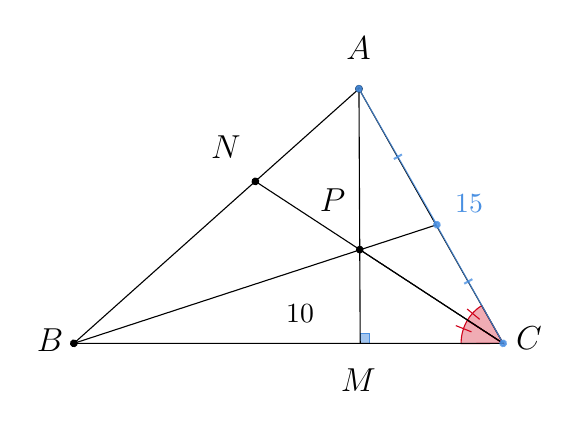
\begin{tikzpicture}[x=0.75pt,y=0.75pt,yscale=-1,xscale=1]
%uncomment if require: \path (0,880); %set diagram left start at 0, and has height of 880

%Shape: Rectangle [id:dp13806740509957183] 
\draw  [color={rgb, 255:red, 74; green, 144; blue, 226 }  ,draw opacity=1 ][fill={rgb, 255:red, 74; green, 144; blue, 226 }  ,fill opacity=0.51 ] (480.97,635.35) -- (485.51,635.35) -- (485.51,639.88) -- (480.97,639.88) -- cycle ;
%Shape: Pie [id:dp047378769040485436] 
\draw  [color={rgb, 255:red, 208; green, 2; blue, 27 }  ,draw opacity=1 ][fill={rgb, 255:red, 208; green, 2; blue, 27 }  ,fill opacity=0.33 ] (529.58,640.13) .. controls (529.58,640.08) and (529.58,640.02) .. (529.58,639.97) .. controls (529.58,635.85) and (530.71,632) .. (532.66,628.75) -- (549.82,639.97) -- cycle ;
%Shape: Pie [id:dp8987475379493] 
\draw  [color={rgb, 255:red, 208; green, 2; blue, 27 }  ,draw opacity=1 ][fill={rgb, 255:red, 208; green, 2; blue, 27 }  ,fill opacity=0.33 ] (532.59,628.87) .. controls (534.31,625.96) and (536.69,623.52) .. (539.5,621.78) -- (549.82,639.97) -- cycle ;
%Straight Lines [id:da6810387691615027] 
\draw    (430.48,561.94) -- (549.82,639.97) ;
\draw [shift={(430.48,561.94)}, rotate = 33.18] [color={rgb, 255:red, 0; green, 0; blue, 0 }  ][fill={rgb, 255:red, 0; green, 0; blue, 0 }  ][line width=0.75]      (0, 0) circle [x radius= 1.34, y radius= 1.34]   ;
%Straight Lines [id:da5413838340116013] 
\draw    (480.75,594.81) -- (549.82,639.97) ;
\draw [shift={(480.75,594.81)}, rotate = 33.18] [color={rgb, 255:red, 0; green, 0; blue, 0 }  ][fill={rgb, 255:red, 0; green, 0; blue, 0 }  ][line width=0.75]      (0, 0) circle [x radius= 1.34, y radius= 1.34]   ;
%Shape: Triangle [id:dp8299957442689323] 
\draw   (480.37,517.33) -- (549.82,639.97) -- (343,639.97) -- cycle ;
%Straight Lines [id:da3748542075425485] 
\draw    (480.37,517.33) -- (480.97,639.88) ;
\draw [shift={(480.37,517.33)}, rotate = 89.72] [color={rgb, 255:red, 0; green, 0; blue, 0 }  ][fill={rgb, 255:red, 0; green, 0; blue, 0 }  ][line width=0.75]      (0, 0) circle [x radius= 1.34, y radius= 1.34]   ;
%Straight Lines [id:da16447337045658683] 
\draw    (343,639.97) -- (517.92,582.82) ;
\draw [shift={(343,639.97)}, rotate = 341.91] [color={rgb, 255:red, 0; green, 0; blue, 0 }  ][fill={rgb, 255:red, 0; green, 0; blue, 0 }  ][line width=0.75]      (0, 0) circle [x radius= 1.34, y radius= 1.34]   ;
%Straight Lines [id:da9245405910807316] 
\draw [color={rgb, 255:red, 74; green, 144; blue, 226 }  ,draw opacity=0.8 ]   (480.37,517.33) -- (517.92,582.82) ;
\draw [shift={(517.92,582.82)}, rotate = 60.17] [color={rgb, 255:red, 74; green, 144; blue, 226 }  ,draw opacity=0.8 ][fill={rgb, 255:red, 74; green, 144; blue, 226 }  ,fill opacity=0.8 ][line width=0.75]      (0, 0) circle [x radius= 1.34, y radius= 1.34]   ;
\draw [shift={(499.14,550.07)}, rotate = 240.17] [color={rgb, 255:red, 74; green, 144; blue, 226 }  ,draw opacity=0.8 ][line width=0.75]    (0,2.24) -- (0,-2.24)   ;
\draw [shift={(480.37,517.33)}, rotate = 60.17] [color={rgb, 255:red, 74; green, 144; blue, 226 }  ,draw opacity=0.8 ][fill={rgb, 255:red, 74; green, 144; blue, 226 }  ,fill opacity=0.8 ][line width=0.75]      (0, 0) circle [x radius= 1.34, y radius= 1.34]   ;
%Straight Lines [id:da6914707979595247] 
\draw [color={rgb, 255:red, 74; green, 144; blue, 226 }  ,draw opacity=0.8 ]   (516.28,580.31) -- (549.82,639.97) ;
\draw [shift={(549.82,639.97)}, rotate = 60.66] [color={rgb, 255:red, 74; green, 144; blue, 226 }  ,draw opacity=0.8 ][fill={rgb, 255:red, 74; green, 144; blue, 226 }  ,fill opacity=0.8 ][line width=0.75]      (0, 0) circle [x radius= 1.34, y radius= 1.34]   ;
\draw [shift={(533.05,610.14)}, rotate = 240.66] [color={rgb, 255:red, 74; green, 144; blue, 226 }  ,draw opacity=0.8 ][line width=0.75]    (0,2.24) -- (0,-2.24)   ;
%Straight Lines [id:da27936519411536453] 
\draw [color={rgb, 255:red, 208; green, 2; blue, 27 }  ,draw opacity=1 ]   (527.04,631.42) -- (534.59,634.44) ;
%Straight Lines [id:da7466400012562466] 
\draw [color={rgb, 255:red, 208; green, 2; blue, 27 }  ,draw opacity=1 ]   (532.48,623.42) -- (538.52,628.4) ;

% Text Node
\draw (480.13,497.8) node  [font=\large]  {$A$};
% Text Node
\draw (331.56,638.42) node  [font=\large]  {$B$};
% Text Node
\draw (562.23,637.61) node  [font=\large]  {$C$};
% Text Node
\draw (416.24,545.55) node  [font=\large]  {$N$};
% Text Node
\draw (480.1,657.72) node  [font=\large]  {$M$};
% Text Node
\draw (467.7,570.99) node  [font=\large]  {$P$};
% Text Node
\draw (451.98,625.5) node    {$10$};
% Text Node
\draw (533.41,572.66) node  [color={rgb, 255:red, 74; green, 144; blue, 226 }  ,opacity=1 ]  {$15$};


\end{tikzpicture}
\end{center}

By angle bisector theorem, $$\dfrac{AN}{15}=\dfrac{NB}{10} \Leftrightarrow \dfrac{AN}{NB} = \dfrac{3}{2}.$$ To make things easier, let us do mass point geometry! \footnote{If you want to know more about mass point geometry, click this \href{https://en.wikipedia.org/wiki/Mass_point_geometry}{link in Wikipedia!}. Also, you can watch this tutorial video from \href{https://www.youtube.com/watch?v=kCSsa2Eze4o}{Dumplet.}} By doing so, we can make the figure like this: 

\begin{center}



\tikzset{every picture/.style={line width=0.75pt}} %set default line width to 0.75pt        

\begin{tikzpicture}[x=0.75pt,y=0.75pt,yscale=-1,xscale=1]
%uncomment if require: \path (0,880); %set diagram left start at 0, and has height of 880

%Shape: Square [id:dp6896027016449073] 
\draw  [color={rgb, 255:red, 74; green, 144; blue, 226 }  ,draw opacity=1 ][fill={rgb, 255:red, 74; green, 144; blue, 226 }  ,fill opacity=0.51 ] (198.52,496.37) -- (203.26,496.37) -- (203.26,501.11) -- (198.52,501.11) -- cycle ;
%Shape: Pie [id:dp043147966793220416] 
\draw  [color={rgb, 255:red, 208; green, 2; blue, 27 }  ,draw opacity=1 ][fill={rgb, 255:red, 208; green, 2; blue, 27 }  ,fill opacity=0.33 ] (249.31,501.37) .. controls (249.31,501.31) and (249.31,501.26) .. (249.31,501.2) .. controls (249.31,496.9) and (250.49,492.88) .. (252.53,489.48) -- (270.46,501.2) -- cycle ;
%Shape: Pie [id:dp045607291247087955] 
\draw  [color={rgb, 255:red, 208; green, 2; blue, 27 }  ,draw opacity=1 ][fill={rgb, 255:red, 208; green, 2; blue, 27 }  ,fill opacity=0.33 ] (252.46,489.6) .. controls (254.26,486.56) and (256.74,484.02) .. (259.68,482.19) -- (270.46,501.2) -- cycle ;
%Straight Lines [id:da8166078113324624] 
\draw    (145.76,419.66) -- (270.46,501.2) ;
\draw [shift={(145.76,419.66)}, rotate = 33.18] [color={rgb, 255:red, 0; green, 0; blue, 0 }  ][fill={rgb, 255:red, 0; green, 0; blue, 0 }  ][line width=0.75]      (0, 0) circle [x radius= 1.34, y radius= 1.34]   ;
%Straight Lines [id:da018094643019893608] 
\draw    (198.29,454) -- (270.46,501.2) ;
\draw [shift={(198.29,454)}, rotate = 33.18] [color={rgb, 255:red, 0; green, 0; blue, 0 }  ][fill={rgb, 255:red, 0; green, 0; blue, 0 }  ][line width=0.75]      (0, 0) circle [x radius= 1.34, y radius= 1.34]   ;
%Shape: Triangle [id:dp03265415036096497] 
\draw   (197.89,373.04) -- (270.46,501.2) -- (54.33,501.2) -- cycle ;
%Straight Lines [id:da740561329484472] 
\draw    (197.89,373.04) -- (198.52,501.11) ;
\draw [shift={(197.89,373.04)}, rotate = 89.72] [color={rgb, 255:red, 0; green, 0; blue, 0 }  ][fill={rgb, 255:red, 0; green, 0; blue, 0 }  ][line width=0.75]      (0, 0) circle [x radius= 1.34, y radius= 1.34]   ;
%Straight Lines [id:da023669207363336664] 
\draw    (54.33,501.2) -- (237.13,441.48) ;
\draw [shift={(54.33,501.2)}, rotate = 341.91] [color={rgb, 255:red, 0; green, 0; blue, 0 }  ][fill={rgb, 255:red, 0; green, 0; blue, 0 }  ][line width=0.75]      (0, 0) circle [x radius= 1.34, y radius= 1.34]   ;
%Straight Lines [id:da6460019494306688] 
\draw [color={rgb, 255:red, 74; green, 144; blue, 226 }  ,draw opacity=0.8 ]   (197.89,373.04) -- (237.13,441.48) ;
\draw [shift={(237.13,441.48)}, rotate = 60.17] [color={rgb, 255:red, 74; green, 144; blue, 226 }  ,draw opacity=0.8 ][fill={rgb, 255:red, 74; green, 144; blue, 226 }  ,fill opacity=0.8 ][line width=0.75]      (0, 0) circle [x radius= 1.34, y radius= 1.34]   ;
\draw [shift={(217.51,407.26)}, rotate = 240.17] [color={rgb, 255:red, 74; green, 144; blue, 226 }  ,draw opacity=0.8 ][line width=0.75]    (0,2.24) -- (0,-2.24)   ;
\draw [shift={(197.89,373.04)}, rotate = 60.17] [color={rgb, 255:red, 74; green, 144; blue, 226 }  ,draw opacity=0.8 ][fill={rgb, 255:red, 74; green, 144; blue, 226 }  ,fill opacity=0.8 ][line width=0.75]      (0, 0) circle [x radius= 1.34, y radius= 1.34]   ;
%Straight Lines [id:da21683509132274925] 
\draw [color={rgb, 255:red, 74; green, 144; blue, 226 }  ,draw opacity=0.8 ]   (235.41,438.85) -- (270.46,501.2) ;
\draw [shift={(270.46,501.2)}, rotate = 60.66] [color={rgb, 255:red, 74; green, 144; blue, 226 }  ,draw opacity=0.8 ][fill={rgb, 255:red, 74; green, 144; blue, 226 }  ,fill opacity=0.8 ][line width=0.75]      (0, 0) circle [x radius= 1.34, y radius= 1.34]   ;
\draw [shift={(252.94,470.03)}, rotate = 240.66] [color={rgb, 255:red, 74; green, 144; blue, 226 }  ,draw opacity=0.8 ][line width=0.75]    (0,2.24) -- (0,-2.24)   ;
%Straight Lines [id:da5890915566883959] 
\draw [color={rgb, 255:red, 208; green, 2; blue, 27 }  ,draw opacity=1 ]   (246.66,492.27) -- (254.55,495.43) ;
%Straight Lines [id:da16743846222578962] 
\draw [color={rgb, 255:red, 208; green, 2; blue, 27 }  ,draw opacity=1 ]   (252.34,483.91) -- (258.66,489.11) ;

% Text Node
\draw (198.43,354.69) node  [font=\large]  {$A$};
% Text Node
\draw (40.42,501.26) node  [font=\large]  {$B$};
% Text Node
\draw (284.7,501.76) node  [font=\large]  {$C$};
% Text Node
\draw (130.77,407.55) node  [font=\large]  {$N$};
% Text Node
